\documentclass[12pt,a4paper]{report}

%MARGINESY
\usepackage[left=3cm, right=2.5cm, top=2.5cm, bottom=2.5cm, headsep=1.2cm]{geometry}

%INTERLINIA
\linespread{1.3}

%Język polski
\usepackage{polski}
\usepackage[utf8]{inputenc}

%tekst matematyczny
\usepackage{amsmath}
\usepackage{amsfonts}
\usepackage{amssymb}
\usepackage{amsthm}

%dodawanie grafiki
\usepackage{graphicx}

%do kolorów
\usepackage{color}
\usepackage{xcolor}

%do numeracji nie od początku
\usepackage{enumitem}

\usepackage{textcomp}%do symbolu euro
\usepackage[official]{eurosym}%drugi symbol euro

%do tabel
\usepackage{tabularx}
\usepackage{multirow} %do połączenia wierszy
\usepackage{diagbox}%do ukośnej linii w tabelii
\usepackage{booktabs}
\usepackage{array}
\newcolumntype{Y}{>{\centering\arraybackslash}X}
\newcolumntype{j}{>{\raggedleft}p{200pt}}
\usepackage{caption}
\usepackage{lscape}

%definicje, twierdzenia,...
\newtheorem{twierdzenie}{Twierdzenie}[chapter]
\newtheorem{lemat}[twierdzenie]{Lemat}
\newtheorem{wniosek}[twierdzenie]{Wniosek}
\newtheorem{obserwacja}[twierdzenie]{Obserwacja}
\newtheorem{uwaga}[twierdzenie]{Uwaga}
\theoremstyle{definition} %prostowanie czcinki
\newtheorem{przyklad}[twierdzenie]{Przykład}
\newtheorem{definicja}[twierdzenie]{Definicja}

%używane pakiety
%\usepackage{setspace}
%\usepackage{cite}
%\usepackage{tikz}
%\usepackage{subcaption}
\usepackage{graphicx}

\usepackage{algorithm}
\usepackage{algpseudocode}
\usepackage{listings}
\usepackage{chngcntr}
\counterwithout{footnote}{chapter}

\definecolor{niebieski}{RGB}{0,130,150} %kolor niebieski
\definecolor{mygray}{gray}{0.6} 		% kolor szary

\lstset{ 
	backgroundcolor=\color{white},   % choose the background color; you must add \usepackage{color} or \usepackage{xcolor}; should come as last argument
	basicstyle=\footnotesize\ttfamily\fontsize{11}{0.8em}\selectfont,        % the size of the fonts that are used for the code
	breakatwhitespace=false,         % sets if automatic breaks should only happen at whitespace
	breaklines=true,                 % sets automatic line breaking
	captionpos=b,                    % sets the caption-position to bottom
	commentstyle=\color{mygreen},    % comment style
	escapeinside={\%*}{*)},          % if you want to add LaTeX within your code
	extendedchars=true,              % lets you use non-ASCII characters; for 8-bits encodings only, does not work with UTF-8
	firstnumber=1,                   % start line enumeration with line 1
	frame=single,	                   % adds a frame around the code
	keepspaces=true,                 % keeps spaces in text, useful for keeping indentation of code (possibly needs columns=flexible)
	keywordstyle=\color{blue},       % keyword style
	numbers=left,                    % where to put the line-numbers; possible values are (none, left, right)
	numbersep=5pt,                   % how far the line-numbers are from the code
	numberstyle=\tiny\color{mygray}, % the style that is used for the line-numbers
	rulecolor=\color{black},         % if not set, the frame-color may be changed on line-breaks within not-black text (e.g. comments (green here))
	showspaces=false,                % show spaces everywhere adding particular underscores; it overrides 'showstringspaces'
	showstringspaces=false,          % underline spaces within strings only
	showtabs=false,                  % show tabs within strings adding particular underscores
	stepnumber=1,                    % the step between two line-numbers. If it's 1, each line will be numbered
	stringstyle=\color{mymauve},     % string literal style
	tabsize=2	                   % sets default tabsize to 2 spaces
}

%parametry dla kodów źródłowych
\definecolor{mygreen}{rgb}{0,0.6,0}
\definecolor{mygray}{rgb}{0.5,0.5,0.5}
\definecolor{mymauve}{rgb}{0.58,0,0.82}

\begin{document}
	%strona tytułowa
	
	\thispagestyle{empty}
	\begin{titlepage}
		\def\dystans{1cm}
		\begin{center}
			\Large 
			\includegraphics[scale=0.8]{prz_pl.png}\\
			Politechnika Rzeszowska 
			im. Ignacego Łukasiewicza\\
			Wydział Matematyki i Fizyki Stosowanej
		\end{center}
		\vspace{1.3cm}
		\begin{center}
			{\Large  \textsc{\textbf{PRACA MAGISTERSKA}} \\
				\vspace{0.5cm}
				\large kierunek studiów: inżynieria i analiza danych }
		\end{center}
		\vspace{1.1cm}
		\begin{center}
			
			{\LARGE\textsc{Analiza i prognozowanie opłat transakcyjnych sieci Bitcoina}}\\
		\end{center}	
		\vspace{1.1cm}
		\begin{center}
			{\Large {inż. Daniel Krzysik}}
		\end{center}
		
		\vspace{1cm} 
		\begin{flushright}		
			\begin{minipage}{0.5\textwidth}
				\begin{flushright}
					\large
					Promotor \\
					dr inż. Dawid Jaworski
				\end{flushright}
			\end{minipage}
		\end{flushright}		
		
		
		\vfill 
		\begin{center}
			{\Large Rzeszów 2025}
		\end{center}
	\end{titlepage}
	
	%spis treści
	\setcounter{tocdepth}{1}
	\tableofcontents
	%\thispagestyle{headings}
	%\setcounter{page}{5}
	
	\chapter*{Wstęp}
	\hspace*{\parindent}Bitcoin, jako pierwsza zdecentralizowana kryptowaluta, zrewolucjonizował podejście do cyfrowego przesyłania wartości bez udziału instytucji pośredniczących. Mechanizmy zawarte w protokole Bitcoina, takie jak nagroda blokowa czy opłaty transakcyjne, decydują o~trwałości i~bezpieczeństwie całego ekosystemu. Wraz z kolejnymi 		halvingami, zmniejszającymi stopniowo liczbę nowo tworzonych bitcoinów w nagrodzie blokowej, rola opłat transakcyjnych staje się coraz większa. Opłaty te nie tylko motywują górników do weryfikacji i~dodawania transakcji do bloków, lecz także regulują przepustowość sieci.

	Niniejsza praca poświęcona jest analizie oraz prognozowaniu opłat transakcyjnych w sieci Bitcoin z uwzględnieniem aspektów technicznych i~ekonomicznych. W rozdziale I~przedstawiono teoretyczne podstawy działania Bitcoina, mechanizm transakcji i~powiązane z nim opłaty, a także omówiono nagrodę dla górników i~znaczenie transakcji coinbase. 			Poruszone zostały kwestie takie jak problem niskiej opłaty czy metody jej podwyższania. Scharakteryzowano również rolę i~konfigurację Bitcoin Core, oficjalnej implementacji protokołu, niezbędnej do praktycznych eksperymentów.

	W rozdziale II przedstawiono proces automatyzacji pobierania oraz przetwarzania danych z łańcucha bloków Bitcoina. Omówiono etapy, takie jak konfiguracja serwera i~środowiska wirtualnego, instalacja Bitcoin Core oraz wykorzystanie interfejsu RPC do gromadzenia bloków i~transakcji. Zaprezentowano także sposób wyodrębniania i~eksportu 		danych do formatu Parquet, co pozwala na bardziej efektywne i~elastyczne zarządzanie dużymi zbiorami informacji.

	Rozdział III koncentruje się na analizie oraz prognozowaniu opłat transakcyjnych w~sieci Bitcoin. Opisano plan projektu bazujący na zbiorze danych wyodrębnionych z~łańcucha bloków oraz informacje o cenie Bitcoina, które posłużyły do przeprowadzenia analiz. Następnie ukazano proces przetwarzania danych: od imputacji brakujących wartości liczbowych, przez inżynierię cech i~skalowanie, po kodowanie zmiennych kategorycznych. W dalszej części rozdziału zaprezentowano porównanie różnych modeli predykcyjnych w ujęciu wielowymiarowym, obejmujących: \textit{Linear Regression}, \textit{Ridge Regression}, \textit{ElasticNet}, \textit{Decision Tree Regressor}, \textit{Random Forest}, \textit{Gradient Boosting} oraz \textit{XGBoost}. Przedstawiono również proces dostrajania hiperparametrów - zarówno w sposób ręczny, jak i z wykorzystaniem narzędzia \textit{GridSearchCV}. Oceny skuteczności dokonano na podstawie metryk RMSE oraz współczynnika determinacji $R^2$. Kolejny etap analizy dotyczył podejścia jednowymiarowego, w którym wykorzystano wyłącznie numer bloku jako zmienną predykcyjną. W tym celu przetestowano dwa modele: regresję liniową oraz model szeregów czasowych SARIMA. Pozwoliło to ocenić, czy struktura czasowa danych (bez dodatkowych cech transakcyjnych) niesie wystarczającą ilość informacji do skutecznego prognozowania opłat.

Zamieszczone w pracy wnioski i~obserwacje mogą stanowić cenną podstawę zarówno dla użytkowników kryptowalut, planujących optymalizację kosztów transakcji, jak i~badaczy, którzy chcą pogłębić wiedzę na temat mechanizmów kształtujących stabilność oraz skalowalność systemów opartych na łańcuchu bloków.
	\addcontentsline{toc}{chapter}{Wstęp}
	
	\chapter{Teoretyczne podstawy i~mechanizmy działania sieci Bitcoina}
	\hspace*{\parindent}Kryptowaluta to wirtualna waluta, wykorzystująca kryptografię do zabezpieczania transakcji. W odróżnieniu od tradycyjnych walut, kryptowaluty nie są kontrolowane przez żaden centralny organ, taki jak bank czy rząd. Działają w oparciu o zdecentralizowaną sieć komputerową, najczęściej wykorzystując technologie 					blockchain\footnote{https://www.kaspersky.com/resource-center/definitions/what-is-cryptocurrency}. Kryptowaluty znajdują zastosowanie w wielu dziedzinach. Na początku miały służyć jako środek płatniczy, bądź forma inwestycji, jednak z czasem ich rola znacznie się rozszerzyła. Pierwszą i~najbardziej znaną kryptowalutą jest Bitcoin (BTC) (\figurename~\ref{fig:logoBTC}). Do walut o największej kapitalizacji rynkowej należą również Ethernum (ETH), Ripple (XRP) czy Solana (SOL). Warto również wspomnieć o tzw. stablecoinach, czyli kryptowalutach powiązanych z wartością walut fiducjarnych (np. USD czy EUR), które charakteryzują się relatywną stabilnością cen. Przykładem stablecoina odwzorowującego kurs polskiego złotego (PLN) jest Omega Złotówka (PLNx), dostępna m. in. na giełdzie Kanga\footnote{https://kanga.exchange}.

\enlargethispage{2\baselineskip}Jednym z ważniejszych zastosowań technologii blockchain są tzw. smart kontrakty (inteligentne kontrakty) - samowykonujące się programy, które automatycznie realizują zaprogramowane warunki w zdecentralizowanym środowisku. Ich działanie nie wymaga pośredników ani zaufania między stonami transakcji, ponieważ warunki kontraktu są jawne, zapisane w kodzie i~niezmienione po wdrożeniu. Smart kontrakty znalazły, szerokie zastosowanie m.in. w zdecentralizowanych finansach (DeFi), w systemach zarządzania tożsamocią, tokenizacji aktywów, grach typu play-to-earn, a także w mechanizmach głosowania i~zarządzania projektami w formie zdecentralizowanych organizacji autonomicznych (DAO).

	\begin{figure}[H]
	    \centering
	    
\includegraphics[width=0.55\textwidth]{../screeny/logoBTC.png} 
	    \caption{Powszechnie używane logo Bitcoina}
	    \label{fig:logoBTC}
	\end{figure}

	Blockchain to rozproszona, publiczna księga, w której dane są zapisywane w postaci bloków, tworząc ciągły łańcuch. Każdy taki blok zawiera zbiór informacji o~transakcji, takich jak metadane, znacznik czasu (timestamp) oraz kryptograficzny skrót (hash) poprzedniego bloku. Każdy blok jest ściśle powiązany z poprzednim, dzięki temu 			system gwarantuje niezmienność i~integralność zapisanych danych\footnote{A. Antonopoulos, D. Harding. Bitcoin. Wszystko, co musisz wiedzieć o programowaniu z użyciem otwartego łańcucha bloków. Wydanie III, 2024. Strona 29/30}. Wykorzystując algorytm proof-of-work odbywa się wydobywanie (mining) - proces dodawania nowego bloku do istniejącego łańcucha bloków. W języku polskim termin \textit{łańcuch bloków} często bywa określany jako \textit{blockchain}, a w dalszej części pracy oba te określenia będą używane zamiennie. W ramach tego procesu bloki w~sieci Bitcoin są dodawane średnio co 10 minut, niezależnie od liczby transakcji czy poziomu aktywności użytkowników. Jest to efekt celowego mechanizmu regulacyjnego, który dostosowuje trudność wydobycia tak, aby utrzymać stałe tempo generowania bloków. Każdy uczestnik sieci, który zainstalował i~uruchomił własny węzeł (node) posiada pełną, lokalną kopię całego blockchaina, co oznacza, że baza danych jest rozproszona i~nie zależy od pojedynczego, centralnego serwera. Taka struktura zapewnia decentralizację, jeśli jakiś węzeł ulegnie awarii lub zostanie zaatakowany, pozostałe utrzymają spójność i~integralność całego systemu. W praktyce, gdy ktoś próbuję zmienić dane w jednym z bloków, zmienia się jego hash, powoduje to rozbieżności w łańcuchu przechowywanym przez inne węzły, a taka nieautoryzowana modyfikacja zostanie natychmiast wykryta i~odrzucona przez sieć. Zabezpieczenia kryptograficzne blockchaina opierają się na algorytmach, takich jak SHA-256, które gwarantują, że obliczenia są nieodwracalne i~trudne do podrobienia.

	Twórca Bitcoina Satoshi Nakamoto (pseudonim anonimowego autora lub grupy osób) opublikował w 2008 roku artykuł: Bitcoin: A Peer-to-Peer Electronic Cash System\footnote{Satoshi Nakamoto. Bitcoin: A Peer-to-Peer Electronic Cash System. 2008.}. Autor rozpoczyna od wskazania problemu jakim jest brak zaufania między stronami, a następnie 			przedstawia koncepcje systemu, w którym transakcje odbywają się bez zaufanego centralnego organu. System ten dodatkowo rozwiązuje problem podwójnego wydawania poprzez wprowadzenie publicznego rejestru łańcucha bloków. 
	
Główna zasada działania proof-of-work (PoW) polega na tym, że aby mieć kontrolę nad siecią, należałoby dysponować ponad 50\% całkowitej mocy obliczeniowej systemu. Teoretycznie umożliwiałoby to przeprowadzenie tzw. ataku 51\%, który mógłby prowadzić do manipulacji sieci, np. podwójnego wydawania środków. W praktyce jednak przejęcie takiej mocy jest niemal niemożliwe ze względu na ogromne rozproszenie górników oraz wysoki koszt energetyczny. Dzięki temu sieć Bitcoina pozostaje bezpieczna i~odporna na manipulacje.

W odróżnieniu od PoW, niektóre nowsze systemy kryptowalut wykorzystują mechanizm proof-of-stake (PoS), w którym zamiast mocy obliczeniowej decydującym czynnikiem jest liczba zgormadzonych tokenów danej kryptowaluty. Uczestnicy sieci są wybierani do tworzenia bloków proporcjonalnie do posiadanych udziałów, co znacząco obniża zapotrzebowanie na energię, ale wprowadza inne wyzwania związane z bezpieczeństwem i~decentralizacją.

Zabezpieczona mechanizmem proof-of-work, każda transakcja jest połączona z poprzednią za pomocą podpisów cyfrowych. Rozwiązaniem jest sieć peer-to-peer, w której uczestnicy (węzły) komunikują się bezpośrednio. Górnicy konkurują w rozwiązywaniu skomplikowanych zagadek kryptograficznych, a w nagrodę otrzymują  nowo wygenerowane bitcoiny i~opłaty transakcyjne, dzięki temu utrzymują prawidłowe działanie sieci. Mechanizm sieci Bitcoin automatycznie dostosowuje trudność tych zagadek matematycznych w zależności od aktualnego obciążenia sieci oraz liczby aktywnych górników. W sytuacji, gdy liczba kopiących wzrasta, zadania stają się bardziej skomplikowane, co skutkuje rzadszym wykopywaniem bloków. Analogicznie, gdy zainteresowanie siecią maleje, trudność zadań jest zmniejszana, tak aby średni czas wydobycia pojedyńczego bloku utrzymywał się na poziomie około 10 minut. Dzięki temu mechanizmowi sieć zachowuje stabilność i~przewidywalność działania.

	Sieć Bitcoina weszła w życie w 2009 roku, co zapoczątkowało funkcjonowanie pierwszej zdecentralizowanej kryptowaluty. Dwa lata później w 2011 roku niespodziewanie zniknął z Internetu Satoshi Nakamoto, pozostawiając aktywnej grupie wolontariuszy odpowiedzialność za dalszy rozwój Bitcoina. Powstanie Bitcoina jest przełomowym osiągnięciem, 			które zapoczątkowało rozwój nowych technologii blockchain i~kryptografii, prowadząc do powstania innowacyjnych rozwiązań w takich dziedzinach jak informatyka czy ekonomia. 
	\section{Bitcoin}
	\hspace*{\parindent} Bitcoin to cyfrowym środek transakcji, oparty na technologii blockchain. Powodem powstania było opracowanie systemu płatniczego, w którym transakcje nie wymagają pośrednictwa osób trzecich takie jak banki czy instytucje rządowe. Bitcoin bazuje na zasadach kryptografii, które umożliwiają zabezpieczenie transakcji oraz 		integralność danych. Transakcje są przetwarzane i~weryfikowane przez uczestników sieci, zwanych węzłami, a wszystkie operacje są zapisywane publicznie w blockchainie.

	Sieć Bitcoina opiera się na technologii blockchain, która stanowi jej fundament, lecz sama sieć to coś więcej niż tylko uporządkowany rejestr transakcji. Blockchain zapisuje dane w blokach, tworząc niezmienny łańcuch, natomiast sieć Bitcoina odpowiada za szybką i~efektywną wymianę informacji między wszystkimi niezależnymi węzłami. Różnica między 		siecią Bitcoin, a blockchainem polega na ich funkcji. Blockchain to niezmienny, statystyczny rejestr transakcji, natomiast sieć Bitcoina odpowiada za przesyłanie, weryfikowane i~synchronizacje w czasie rzeczywistym. Dzięki otwartemu protokołowi, możliwe jest natychmiastowe rozsyłanie nowych transakcji i~bloków między uczestnikami, 					sprawia to, że każdy komputer posiada aktualną, spójną wersję rejestru, niezależnie od lokalizacji, a brak centralnego serwera zapewnia odporność na ataki i~awarie.

	Kluczowym elementem działania sieci Bitcoin jest ochrona przed podwójnym wydatkowaniem. Podczas, gdy użytkownik rozpoczyna transakcje, informacja ta zostaje rozsyłana do wszystkich węzłów, które sprawdzają, czy środki nie zostały wcześniej użyte. Dzięki temu każda próba wykorzystania tych samych bitcoinów w więcej niż jednej transakcji 			zostaje natychmiastowo wykryta, co stanowi fundament bezpieczeństwa całego systemu.
	\section{Transakcje i~opłaty transakcyjne}
	\hspace*{\parindent} Transakcje to cyfrowe operacje, polegające na przesyłaniu środków między różnymi adresami w sieci. Każda transakcja składa się z wejść (input), które wskazują źródło pochodzących środków z poprzednich transakcji oraz wyjść (outputs), które określają odbiorców czyli, na jakie adresy i~w jakiej kwocie mają trafić środki. Śledzenie 			przepływu środków i~zapewnienie spójności historii transakcji jest możliwe dzięki takiej strukturze.

	Decydującą aspektem transakcji jest ich bezpieczeństwo, polega to na tym, że każda operacja jest podpisywana cyfrowo przez właściciela portfela. Umożliwia to niezależna weryfikacje autentyczności przez innych uczestników systemu. W przeciwieństwie do tradycyjnych przelewów bankowych, które mogą być cofnięte, zatwierdzenie transakcji przez sieć  	i~dodanie jej do blockchaina, oznacza, że operacja staje się nieodwracalna. Zapobiega to próbom ponownego wykorzystania tych samych środków i~chroni system przed oszustwami\footnote{A. Antonopoulos, D. Harding. Bitcoin. Wszystko, co musisz wiedzieć o programowaniu z użyciem otwartego łańcucha bloków. Wydanie III, 2024. Strona 207}.
	Opłaty transakcyjne to niewielkie dodatkowe koszty, które użytkownicy mogą dołączać do swoich transakcji w sieci. Stanowią zachętę dla górników, którzy zatwierdzają transakcje i~dodają je do blockchaina. W praktyce oznacza to, im wyższa opłata, tym większa szansa, że transakcja zostanie szybko uwzględniona w~nowym bloku. W okresach dużego przeciążenia jest to szczególnie ważne.

	W sieci Bitcoina górnicy otrzymują wynagrodzenie za dodanie nowego bloku do łańcucha. Jest nim tzw. nagroda blokowa (block reward), która początkowo wynosiła 50 BTC. Nagroda składa się z dwóch części: nowych bitcoinów wygenerowanych w~momencie wydobycia bloku oraz sumy opłat transakcyjnych zawartych w tym bloku. Nowo wygenerowane bitcoiny pełnią funkcję mechanizmu emisji i~są jedynym sposobem wprowadzenia nowych jednostek tej kryptowaluty do obiegu.

	Zgodnie z założeniami protokołu Bitcoina, nagroda bokowa zmniejsza się o połowę co 210 000 bloków, czyli średnio co około cztery lata. To zjawisko określane jest jako halving. Ma ono na celu stopniowe ograniczenie podaży nowych bitcoinów, co stanowi zabezpieczenie przed inflacją. Po pierwszym halvingu w 2012 roku nagroda spadła z 50 BTC do 25 BTC, a obecnie po piątym halvingu, który miał miejsce w kwietniu 2024 roku wynosi już tylko 3,125 BTC. Proces ten będzie kontynuowany, aż do osiągniecia maksymalnej liczby 21 milionów bitcoinów, co zgodnie z szacunkami nastąpi około roku 2140. 

	Aktualne zapotrzebowanie sieci dynamicznie wpływa na wysokość opłat transakcyjnych. Górnicy wybierają priorytetowe transakcje do przetworzenia, czyli te, w których użytkownik zaproponował wyższa opłatę. W momencie, gdy suma wartości środków wejściowych przekracza wartość środków wyjściowych, różnica ta stanowi opłatę transakcyjną, która trafia do górnika, zatwierdzającego dany blok. W momencie, kiedy nagroda za wydobycie nowych bloków stopniowo maleje, istotnym źródłem dochodu dla górników stają się opłaty transakcyjne\footnote{https://www.bitcoin.com/get-started/what-are-crypto-network-fees/}. W systemie Bitcoina (BTC) opłata transakcyjna pełni ważną rolę, gdyż, przede wszystkim jest motywacją dla górników, która stanowi dodatkowe wynagrodzenia poza nagrodą blokową. Nagroda blokowa zmniejsza się w~czasie, dlatego opłaty transakcyjne zyskują na znaczeniu jako istotne źródło dochodu, co wspiera bezpieczeństwo i~stabilność sieci. Dodatkowo, mechanizm opłat działa jak bariera ochronna przed atakami spamowymi, zniechęcając do wysyłania dużej liczby drobnych i~niepotrzebnych transakcji, które mogłyby przeciążyć sieć.

	\section{Nagroda dla górników i~transakcja coinbase}
	\hspace*{\parindent}Górnicy otrzymują dwa wynagrodzenia: nagrody blokowej, czyli nowo stworzone bitcoiny przyznane za dodanie bloku do blockchaina oraz opłat transakcyjnych. Transakcja coinbase to specjalny rodzaj operacji, gdyż zawsze pojawia się jako pierwsza w~nowo wykopanym bloku. Jej głównym celem jest utworzenie nowych bitcoinów, a~górnikowi przyznanie nagrody blokowej. W odróżnieniu od zwykłych transakcji nie posiada danych wejściowych, wynika to z faktu, że nie wykorzystuje środków z poprzednich transakcji. Opłata transakcyjna w transakcji coinbase często wynosi 0, gdyż jej głównym zadaniem jest wytworzenie nowych bitcoinów.
	\section{Jednostki opłat transakcyjnych}
	\hspace*{\parindent}Obecnie najczęściej opłaty za przesyłanie środków w sieci Bitcoin są wyrażane w~satoshi – najmniejszej jednostce tej kryptowaluty, gdzie 1 BTC odpowiada za 100 milionom satoshi. Stosuje się jednostki, takie jak satoshi za baj (sat/B) lub satoshi za wirtualny bajt (sat/vB), które umożliwiają dokładne dostosowanie opłaty do rozmiaru 			transakcji\footnote{Tangem Team. Bitcoin Transaction Fees. Tangem Blog, 2021.}. 
	\section{Podwyższanie opłat – co zrobić, gdy transakcja utknie?}
	\hspace*{\parindent}\enlargethispage{2\baselineskip}Nadawca może ustalić zbyt niską opłatę transakcyjną, dana operacja może pozostawać w \textit{mempoolu} – w zbiorze niezatwierdzonych transakcji, które oczekują na dodanie do bloku. Szczególnie w okresach dużego obciążenia sieci, możemy spotkać się z tą sytuacją, gdyż górnicy dążą do maksymalizacji zysków\footnote{FAQ Mempool Documentation, 2023.}.
	\subsection{Mechanizm podwyższania opłaty}
	\hspace*{\parindent}W sytuacjach, kiedy transakcja utknie w mempoolu, użytkownik ma możliwość skorzystania z metod podwyższania opłat, które to staną się bardziej atrakcyjne dla górnika. Wyróżnia się dwa rozwiązania\footnote{Greg Walker. Learn Me A Bitcoin, 2021.}:
\begin{itemize}
	\item \textbf{Replace-by-Fee (RBF)} – pozwala na zastąpienie oczekującej transakcji nową wersją, w której będzie wyższa opłata.
	\item \textbf{Child Pays for Parent (CPFP)} – ta metoda wysyła dodatkową, powiązaną transakcję o wysokiej opłacie, która zachęca górnika do zatwierdzenia zarówno nowej \textit{dziecięcej}, jak i~nadrzędnej \textit{rodzicielskiej} o niższej opłacie. 
\end{itemize}
	\section{Dynamika i~przyszłość opłat transakcyjnych}
	\hspace*{\parindent}Wysokość opłat jest dynamiczna i~zależy w głównej mierze od obciążenia sieci. Wraz ze wzrostem liczby transakcji i~rosnącą konkurencją o miejsce w bloku, opłaty zwykle rosną, ponieważ użytkownicy starają się przyspieszyć przetworzenie swoich operacji. W~okresach mniejszego ruchu, opłaty zwykle spadają. W wyniku halvingu 			nagrody blokowe 	spadają, zatem w przyszłości opłaty transakcyjne mogą stać się jeszcze ważniejszym źródłem dochodu dla górników, co wypłynie na ich wysokość. Ostateczny kształt zmian będzie uzależniony nie tylko od wzrostu liczby użytkowników i~technologii, ale również od czynników zewnętrznych, takich jak rozgłos medialny, ceny Bitcoina, zmieniające się regulacje dotyczące kryptowalut, a także od ewolucji podstaw kryptografii oraz potencjalnych aktualizacjach protokołu Bitcoina, zwanych hard forkami\footnote{https://cryptomus.com/pl/blog/what-is-a-hard-fork-in-cryptocurrency}.  
	\section{Bitcoin Core}
	\hspace*{\parindent} Bitcoin Core to oficjalne oprogramowanie open-source, które stanowi implementacje protokołu Bitcoin. Działa jako pełny węzeł (full node) w sieci Bitcoin. Umożliwia pobranie, przechowywanie i~weryfikację całej historii transakcji (blockchain), dzięki temu użytkownicy niezależnie mogą sprawdzić poprawność transakcji i~bloków. 			Dodatkowo, Bitcoin Core udostępnia interfejs RPC (Remote Procedure Call), który umożliwia zdalne wysyłanie poleceń do węzła. Pozwala to na automatyzację operacji, takich jak pobieranie danych z blockchaina czy wysyłanie transakcji\footnote{A. Antonopoulos, D. Harding. Bitcoin. Wszystko, co musisz wiedzieć o programowaniu z użyciem 				otwartego łańcucha bloków. Wydanie III, 2024. Strona 52-53}.
	\begin{figure}[H]
	    \centering
	    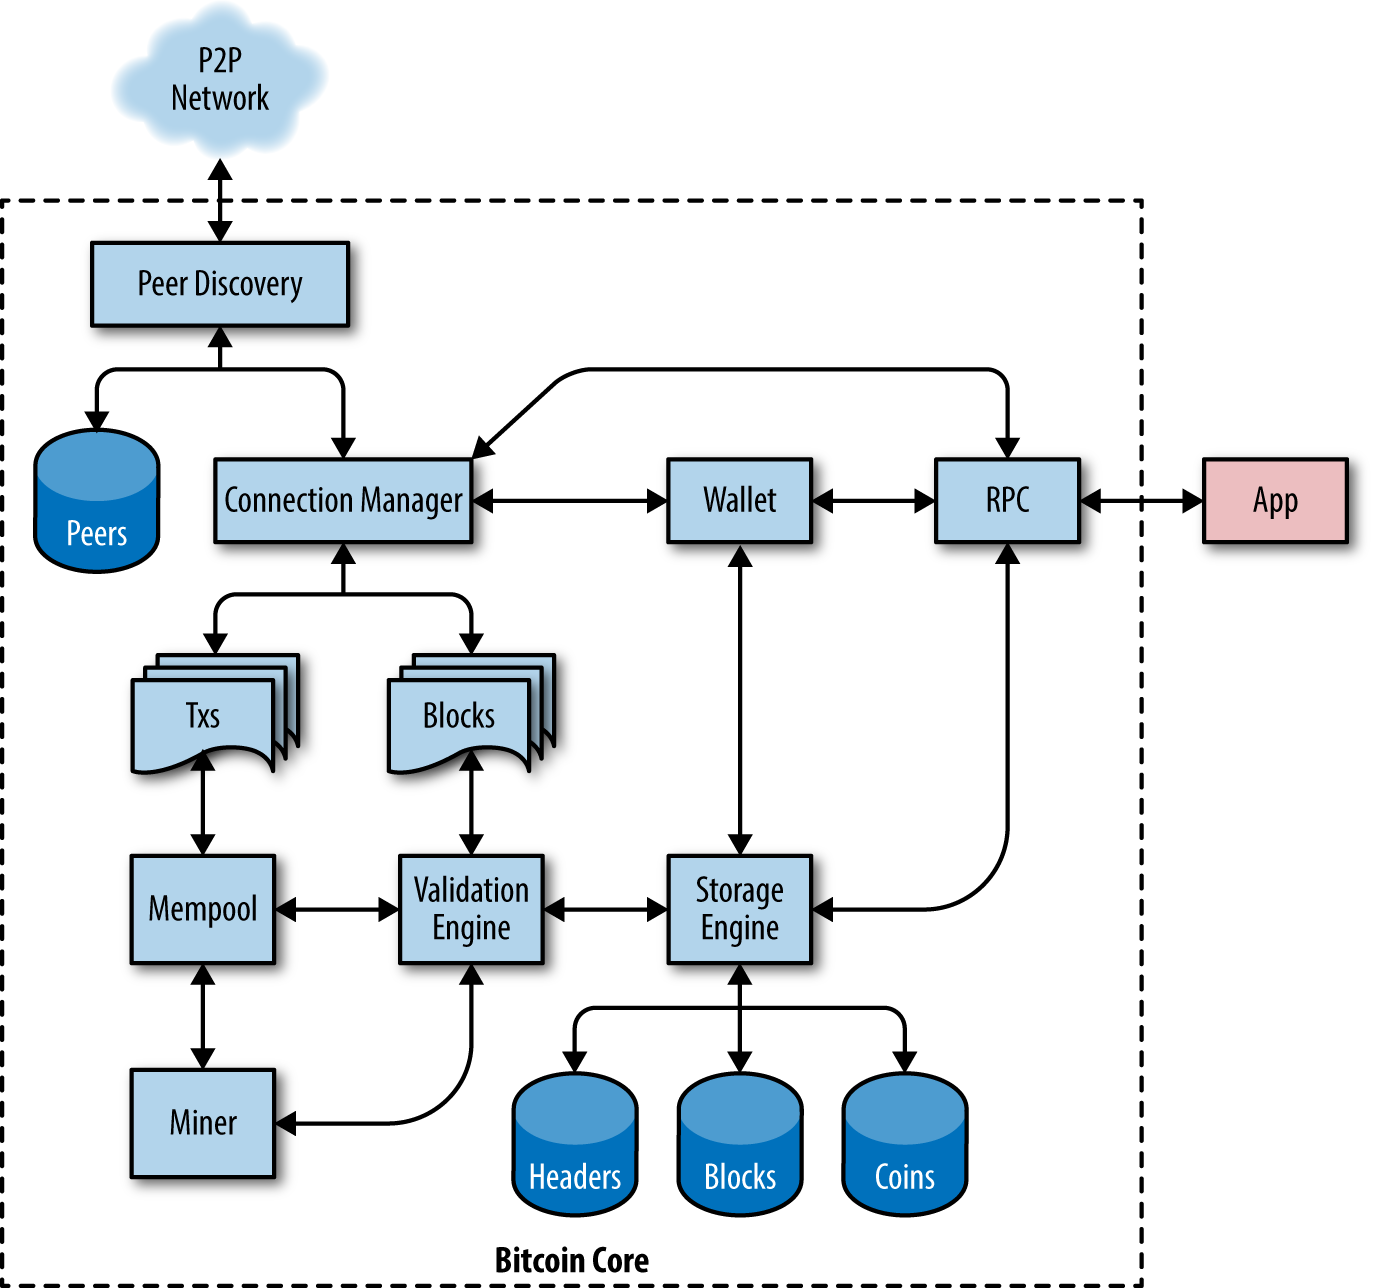
\includegraphics{../screeny/Architektura_Bitcoin_Core.png} 
	    \caption{Architektura implementacji Bitcoin Core (źródło: Eric Lombrozo\protect\footnotemark)}
	    \label{fig:architektura}
	\end{figure}
	\footnotetext{https://cypherpunks-core.github.io/bitcoinbook/ch03.html}
	Diagram (\figurename~\ref{fig:architektura}) przedstawia kluczowe komponenty Bitcoin Core i~ich współpracę w sieci P2P. Peer Discovery (wykrywanie węzłów) oraz Connection Manager (menedżer połączeń) odpowiadają za wyszukiwanie węzłów i~utrzymanie połączeń z~innymi węzłami, podczas gdy Mempool (pula transakcji) i~Validation Engine (system walidacji) przechowują i~weryfikują transakcję. Zatwierdzone dane zapisywane są w~Storage Engine (system przechowywania), a~moduł Wallet (portfel) zarządza środkami użytkownika. Interfejs RPC pozwala na zdalne sterowanie węzłem oraz integracje z~innymi aplikacjami.
	
	\chapter{Automatyzacja pozyskiwania i~przetwarzania danych z łańcucha bloków Bitcoina}
	\hspace*{\parindent}W tym rozdziale opisano w pełni zautomatyzowany proces pozyskiwania i~wstępnej obróbki danych z blockchaina Bitcoina. Analiza opłat transakcyjnych wymagała uruchomienia pełnego węzła, czyli pobrania i~zweryfikowania całego łańcucha bloków. Całość zrealizowano na zewnętrznym serwerze udostępnionym przez Koło 				Naukowe Machine Learning Politechniki Rzeszowskiej, z którym połączono się przez VPN. Na serwerze, utworzono środowisko wirtualne \textit{venv}, zainstalowano klienta Bitcoin Core oraz zautomatyzowano pobieranie bloków poprzez interfejs RPC. Kolejno, za pomocą skryptów w pythonie, wykonano ekstrakcję oraz weryfikację kluczowych danych z łańcucha bloków, które następnie zostały przekształcone i~zapisane w formacie parquet, co pozwoliło na efektywną i~skalowalną analizę danych.
	\section{Pozyskanie danych z blockchaina Bitcoin przy użyciu Bitcoin RPC}
	\hspace*{\parindent} Jednym z najpopularniejszych sposobów na pobieranie danych z łańcucha bloków (blockchaina) Bitcoina jest skorzystanie z Bitcoin RPC (Remote Procedure Call). Bitcoin Core – oficjalna implementacja protokołu Bitcoin – udostępnia interfejs RPC, który pozwala na wykonywanie zdalnych poleceń, takich jak pobieranie informacji o~blokach, transakcjach czy stanie sieci. Dzięki temu można łatwo integrować węzeł Bitcoin z własnymi skryptami czy aplikacjami w celu automatycznego gromadzenia i~przetwarzania danych.

	\subsection{Konfiguracja środowiska pracy}
	\hspace*{\parindent}Pierwszym krokiem w przygotowaniu do pracy było nawiązanie zdalnego i~bezpiecznego połączenia z serwerem Koła Naukowego Machine Learning Politechniki Rzeszowskiej. W tym celu wykorzystano technologię VPN (Virtual Private Network), czyli wirtualną sieć prywatną, która umożliwia stworzenie zaszyfrowanego tunelu komunikacyjnego pomiędzy komputerem użytkownika a serwerem. Dzięki temu połączenie jest chronione przed podsłuchiwaniem i~atakami zewnętrznymi, a transmisja danych odbywa się w sposób poufny i~bezpieczny (\figurename~\ref{fig:ekran2}).

	\begin{figure}[H]
	    \centering
	    \includegraphics[width=0.95\textwidth]{../screeny/VPN\_connection2.jpg} 
	    \caption{Ekran aktywnego połączenia VPN}
	    \label{fig:ekran2}
	\end{figure}

	Kolejnym etapem było przygotowanie środowiska programistycznego na serwerze. Zgodnie z polityką bezpieczeństwa serwera, bezpośrednia instalacja potrzebnych bibliotek była niemożliwa. Aby móc korzystać z niezbędnych narzędzi i~pakietów, utworzono środowisko wirtualne \textit{venv}. Środowisko to pozwala na izolację instalowanych bibliotek i~konfiguracji od globalnego systemu, dzięki czemu zmiany wprowadzone w ramach \textit{venv} nie wpływają na inne aplikacje ani ustawienia serwera. Takie podejście gwarantuje większe bezpieczeństwo, elastyczność oraz możliwość zarządzania zależnościami w~projekcie niezależnie od systemu operacyjnego.

	\subsection{Instalacja Bitcoin Core}
\hspace*{\parindent}Aby analizować możliwie najbardziej aktualny łańcuch bloków, zainstalowano najnowszą wersję Bitcoin Core. Oprogramowanie zostało pobrane z oficjalnej strony (lub repozytorium GitHub), a następnie zainstalowane w przygotowanym wcześniej środowisku wirtualnym. Po zakończeniu tego procesu w katalogu \texttt{/bin} pojawiły się pliki wykonywalne (\figurename~\ref{fig:strukturaBCore}), takie jak \texttt{bitcoind}, \texttt{bitcoin-cli} i~inne.

	\begin{figure}[H]
	    \centering
	    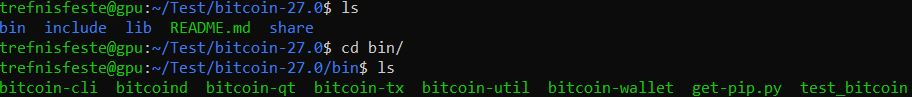
\includegraphics[width=0.99\textwidth]{../screeny/inst1.jpg} 
	    \caption{Struktura katalogów i~plików Bitcoin Core}
	    \label{fig:strukturaBCore}
	\end{figure}

	Węzeł, który przechowuje pełny blockchain Bitcoina od jego powstania w 2009 roku, zajmuje około 744 GB przestrzeni dyskowej (\figurename~\ref{fig:rozmiarBTC}). Początkowa synchronizacja, czyli pobranie całej historii bloków, może trwać od kilkunastu godzin do kilku dni – wszystko zależy od szybkości połączenia internetowego. W przypadku 			utraty połączenia lub innych zakłóceń, po ponownym nawiązaniu łączności węzeł automatycznie aktualizuje się, pobierając brakujące bloki i~przywracając pełną synchronizację z siecią. Ze względu na duże obciążenie serwera innymi procesami członków Koła Naukowego, w opisywanym przypadku proces pełnej synchronizacji trwał około 36 godzin.

	\begin{figure}[H]
	    \centering
	    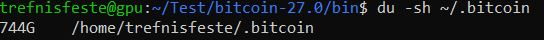
\includegraphics[width=0.75\textwidth]{../screeny/waga_blockchain.jpg} 
	    \caption{Rozmiar blockchaina Bitcoina}
	    \label{fig:rozmiarBTC}
	\end{figure}

	\subsection{Konfiguracja pliku bitcoin.conf}
	\hspace*{\parindent}Zdalna komunikacja przez interfejs RPC została umożliwiona poprzez utworzenie pliku konfiguracyjnego \texttt{bitcoin.conf}\footnote{A. Antonopoulos, D. Harding. Bitcoin. Wszystko, co musisz wiedzieć o programowaniu z użyciem otwartego łańcucha bloków. Wydanie III, 2024. Strona 60}, który pełni funkcję głównego pliku konfiguracyjnego klienta Bitcoin Core. Umożliwia on dostosowanie działania węzła do własnych potrzeb, w tym m.in. aktywację trybu serwera, zarządzanie dostępem do interfejsu RPC oraz włączenie dodatkowych funkcji analitycznych.
	
	\begin{figure}[H]
	    \centering
	    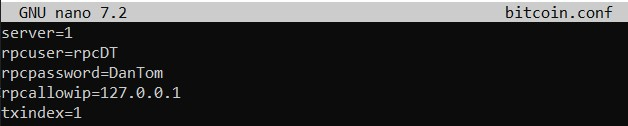
\includegraphics[width=0.95\textwidth]{../screeny/bitcoin_conf.jpg} 
	    \caption{Konfiguracja pliku bitcoin.conf}
	    \label{fig:bitcoinCONF}
	\end{figure}
	
	Niezbędne opcje pliku konfiguracyjnego bitcoin.conf (\figurename~\ref{fig:bitcoinCONF}) to: \texttt{server=1} uruchamia węzeł w trybie serwera; \texttt{rpcuser} oraz \texttt{rpcpassword} określają dane uwierzytelniające do komunikacji RPC; \texttt{rpcallowip=127.0.0.1} zezwala na połączenia RPC z localhost; \texttt{txindex=1} włącza 				indeksowanie transakcji, czyli tworzenie specjalnej bazy danych umożliwiającej szybkie wyszukiwanie i~dostęp do informacji o~dowolnej transakcji w całym łańcuchu bloków. Bez tej opcji klient Bitcoin Core musiałby przeszukiwać wszystkie bloki i~transakcje liniowo, co jest czasochłonne i~nieefektywne. Włączenie indeksowania przyspiesza zapytania dotyczące historii transakcji i~jest niezbędne do zaawansowanych analiz oraz korzystania z niektórych narzędzi zewnętrznych.

	Procesem odpowiedzialnym za pobieranie danych i~synchronizację z siecią Bitcoin jest \texttt{bitcoind}.  Po uruchomieniu inicjuje on pobieranie oraz weryfikację całego łańcucha bloków, dzięki czemu lokalna kopia pozostaje w pełnej zgodności z siecią Bitcoin. Przy jego uruchomieniu należy wskazać katalog danych, w którym zapisane są pliki blockchaina, np.
	\begin{center}
	\textit{./bitcoind -datadir=/home/username/.bitcoin}
	\end{center}

	Po zakończeniu inicjalizacji węzła sprawdzono, czy uruchomione oprogramowanie odpowiada oczekiwanej wersji. Informację tę uzyskano poleceniem:
	\begin{center}
	\textit{./bitcoin-cli –version}
	\end{center}

	\begin{figure}[H]
	    \centering
	    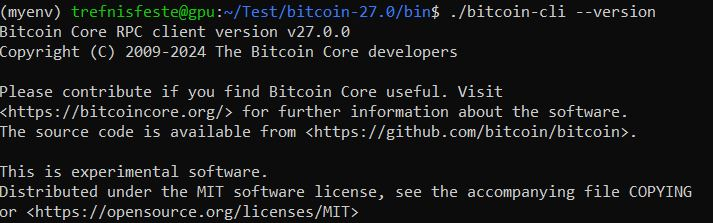
\includegraphics[width=0.95\textwidth]{../screeny/bitcoin-cli-version.jpg} 
	    \caption{Weryfikacja zainstalowanej wersji Bitcoin Core}
	    \label{fig:version}
	\end{figure}
	
	\noindent Wynik potwierdził, że środowisko pracuje w oparciu o Bitcoin Core v27.0.0 (\figurename~\ref{fig:version}).

	Wszelkie modyfikacje parametrów w pliku bitcoin.conf wymagają uprzedniego zatrzymania procesu \textit{bitcoind ./bitcoin-cli stop}, a następnie ponownego uruchomienia Bitcoin Core poleceniem \textit{./bitcoind -daemon}. Zapewnia to, że zaktualizowane ustawienia, zostaną załadowane podczas ponownej inicjalizacji węzła.

	Stan synchronizacji monitorowano za pomocą komendy: \textit{./bitcoin-cli getblockchaininfo}

	\begin{figure}[H]
	    \centering
	    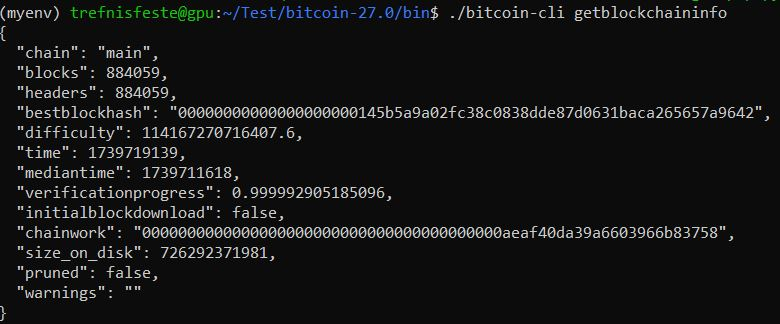
\includegraphics[width=0.95\textwidth]{../screeny/blockchain-info.JPG}
	    \caption{Informacje o stanie blockchaina}
	    \label{fig:blockchainINFO}
	\end{figure}	

	Polecenie zwraca zestaw kluczowych metryk węzła (\figurename~\ref{fig:blockchainINFO}). Wyświetlane wartości obejmują m.in. bieżącą liczba bloków (blocks), wskaźnik postępu weryfikacji (verificationprogress) oraz całkowity rozmiar danych na dysku (size\_on\_disk), pozwalając na bieżącą kontrolę postępu pobierania i~integralności lokalnej kopii 			blockchaina.

	\section{Wyodrębnienie i~eksport danych}
	\hspace*{\parindent}Analiza danych z blockchaina Bitcoina wymaga wyodrębnienia interesujących nas informacji, takich jak numery bloków, wartości transakcji czy opłaty. W tym celu został przygotowany skrypt wykorzystujący interfejs RPC Bitcoin Core, który pobiera szczegółowych danych o każdym bloku i~transakcji w nim zawartych. 

Początkowo dane były zapisywane do plików CSV, co przy dużej liczbie transakcji i~bloków skutkowało znacznymi rozmiarami plików (\figurename~\ref{fig:rozmiarCSV}) i~wydłużonym czasem przetwarzania. Aby zredukować rozmiary plików, zdecydowano się na zapisywanie danych w formacie Parquet, kolumnowym standardzie open-source, który dzięki wbudowanej kompresji i~przechwytywaniu danych kolumna po kolumnie zapewnia mniejszy rozmiar plików oraz szybszy dostęp do informacji.

	\begin{figure}[H]
	    \centering
	    \includegraphics[width=0.9\textwidth]{../screeny/wagi\_csv.jpg} 
	    \caption{Rozmiar plików w formacie CSV}
	    \label{fig:rozmiarCSV}
	\end{figure}

	\subsection{Eksport danych blockchain do formatu Parquet}
	\hspace*{\parindent}Ze względu na problem dużych plików generowanych przy zapisie danych w formacie CSV, zdecydowano się na wdrożenie formatu Parquet, który oferuje lepszą kompresję i~szybszy dostęp do informacji. W kodzie przedstawiono proces pobierania danych za pomocą interfejsu RPC, ich przetwarzanie i~zapis do pliku Parquet.

	Kod \textbf{Pobierz\_Bloki\_V4.py} łączy się z węzłami Bitcoin Core za pomocą interfejsu RPC, a następnie iteracyjnie przetwarza bloki w~żądanym zakresie. Dla każdego bloku pozyskiwane są dane o transakcjach, w tym wartości wejść, wyjść, opłaty oraz nagrody blokowe. W przypadku problemów z połączeniem stosowany jest mechanizm ponawiania prób 		(retry). Dane są gromadzone w formacie listy, a następnie konwertowane do ramki danych przy użyciu biblioteki pandas. W celu ułatwienia analizy i~oszczędności miejsca, ramka danych jest zapisywana w formacie Parquet. Skrypt przetwarza bloki w~zdefiniowanych zakresach, początkowo co 50000, a w miarę wzrostu rozmiaru danych zakres zmniejszono 	do 25000, zapisując logi z wykonania każdej partii.

	\begin{table}[H]
	    \centering
	    \begin{tabular}{|l|l|l|l|}
	        \hline
	        Zakres bloków & Czas rozpoczęcia & Czas zakończenia & Czas trwania \\ \hline
	        0-50000 & 2025-02-16 15:45:23 & 2025-02-16 15:46:04 & 40.77 sekund \\ \hline
	        50001-100000 & 2025-02-16 15:46:05 & 2025-02-16 15:49:05 & 180.17 sekund \\ \hline
	        100001-150000 & 2025-02-16 15:49:06 & 2025-02-16 16:33:53 & 1476.40 sekund \\ \hline
	        200001-250000 & 2025-02-16 16:37:36 & 2025-02-16 17:33:58 & 3381.80 sekund \\ \hline
	        250001-275000 & 2025-02-16 20:45:23 & 2025-02-16 21:13:38 & 1694.52 sekund \\ \hline
	        275001-300000 & 2025-02-17 02:33:41 & 2025-02-17 03:10:01 & 2179.86 sekund \\ \hline
	        300001-325000 & 2025-02-17 12:54:12 & 2025-02-17 13:39:05 & 2693.08 sekund \\ \hline
	        325001-350000 & 2025-02-17 13:54:26 & 2025-02-17 15:01:02 & 3995.92 sekund \\ \hline
	        350001-375000 & 2025-02-17 15:01:05 & 2025-02-17 16:40:41 & 5975.66 sekund \\ \hline
	        375001-400000 & 2025-02-17 16:40:44 & 2025-02-17 18:56:43 & 8159.23 sekund \\ \hline
	        400001-425000 & 2025-02-17 19:50:51 & 2025-02-17 22:50:43 & 10792.66 sekund \\ \hline
	        425001-450000 & 2025-02-17 22:50:46 & 2025-02-18 02:18:48 & 12481.74 sekund \\ \hline
	        450001-475000 & 2025-02-18 02:18:51 & 2025-02-18 06:27:17 & 14906.32 sekund \\ \hline
	        475001-500000 & 2025-02-18 06:27:20 & 2025-02-18 10:21:54 & 14073.13 sekund \\ \hline
	        500001-525000 & 2025-02-18 10:21:57 & 2025-02-18 13:44:58 & 12181.62 sekund \\ \hline
	        525001-550000 & 2025-02-18 13:45:01 & 2025-02-18 16:55:26 & 11424.74 sekund \\ \hline
	        550001-575000 & 2025-02-18 17:31:42 & 2025-02-18 21:49:04 & 15442.05 sekund \\ \hline
	        575001-600000 & 2025-02-18 21:49:07 & 2025-02-19 02:06:06 & 15419.33 sekund \\ \hline
	        600001-625000 & 2025-02-19 12:35:26 & 2025-02-19 16:30:06 & 14079.54 sekund \\ \hline
	        625001-650000 & 2025-02-19 16:30:09 & 2025-02-19 20:57:45 & 16056.41 sekund \\ \hline
	        650001-675000 & 2025-02-19 20:57:48 & 2025-02-20 01:49:03 & 17475.33 sekund \\ \hline
	        675001-700000 & 2025-02-20 01:49:06 & 2025-02-20 05:52:02 & 14576.12 sekund \\ \hline
	        700001-725000 & 2025-02-20 06:49:43 & 2025-02-20 10:52:00 & 14536.42 sekund \\ \hline
	        725001-750000 & 2025-02-24 21:18:42 & 2025-02-25 01:26:50 & 14887.24 sekund \\ \hline
	        750001-775000 & 2025-02-25 01:26:53 & 2025-02-25 05:40:24 & 15211.57 sekund \\ \hline
	        775001-800000 & 2025-02-25 05:40:27 & 2025-02-25 11:56:06 & 22538.61 sekund \\ \hline
	        800001-825000 & 2025-02-25 11:56:09 & 2025-02-25 19:47:04 & 28254.56 sekund \\ \hline
	        825001-850000 & 2025-02-25 19:47:07 & 2025-02-26 03:46:13 & 28746.27 sekund \\ \hline
	        850001-875000 & 2025-02-26 03:46:16 & 2025-02-26 13:30:16 & 35040.09 sekund \\ \hline
	    \end{tabular}
	    \caption{Czas przetwarzania paczek bloków}
	    \label{fig:tabela}
	\end{table}

	\enlargethispage{2\baselineskip}Cały proces wyodrębniania wyniósł łącznie prawie 100 godzin (\tablename~\ref{fig:tabela}, \figurename~\ref{fig:zakresBlokow}), a łączny rozmiar pobranych danych wynosi około 90 GB zapisanych w formacie Parquet. Pierwsza paczka danych, oznaczona jako \textit{dane\_0\_50000.parquet} zawiera informacje o blokach z początku istnienia sieci Bitcoin (styczeń 2009 rok), natomiast ostatnia paczka \textit{dane\_850001\_875000.parquet} obejmuje dane z grudnia 2024 roku. 

	\begin{figure}[H]
	    \centering
	    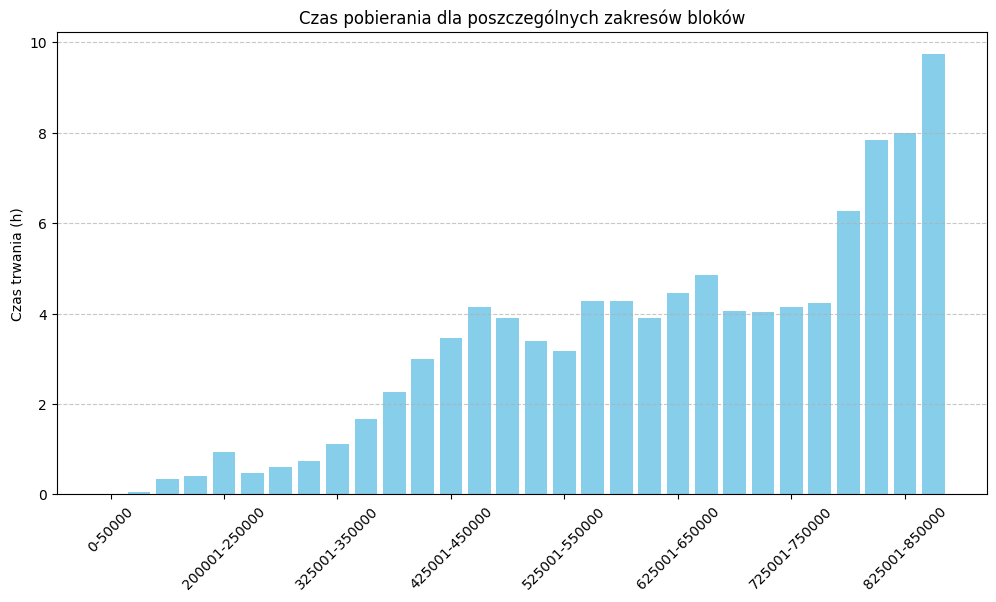
\includegraphics[width=0.95\textwidth]{../screeny/czas_pobierania.png} 
	    \caption{Czas pobierania dla poszczególnychn zakresów bloków}
	    \label{fig:zakresBlokow}
	\end{figure}
	
	Wczytanie kilkudziesięciu gigabajtów danych w każdym kroku analizy może być trudne do utrzymania zarówno pod względem pamięci operacyjnej, jak i~czasu obliczeniowego. W kontekście przeprowadzanej analizy nie jest konieczne przetwarzanie całego zbioru danych, dlatego zdecydowano się na utworzenie próbki o wielkości 1\% całego zbioru.
	
	Skrypt \textbf{Pobierz\_Probke.py} działa w następujący sposób: najpierw przeszukuje katalog w poszukiwaniu wszystkich plików z rozszerzeniem .parquet (\figurename~\ref{fig:rozmiarParquet}), zachowując chronologiczną kolejność od najwcześniejszych do najnowszych danych. Każdy plik zawiera dane transakcji z~określonego okresu (bloków blockchain). Następnie, dla każdego pliku, losowo wybierane jest 1\% wierszy, czyli pojedynczych transakcji. Dzięki temu próbka odzwierciedla charakterystyki transakcji z~danego okresu. Ważne jest, że próbkujemy transakcje, a nie całe bloki, ponieważ liczba transakcji na blok rośnie w~czasie, późniejsze pliki (z nowszymi blokami) zawierają więcej transakcji, więc mają też proporcjonalnie większy udział w finalnej próbce. Ostatecznie próbki transakcji z~kolejnych plików są scalane w jeden zbiór, który stanowi uporządkowany chronologicznie, losowy podzbiór wszystkich danych. Tak przygotowany plik umożliwia efektywną i~reprezentatywną analizę bez konieczności przetwarzania całego zbioru.

	\begin{figure}[H]
	    \centering
	    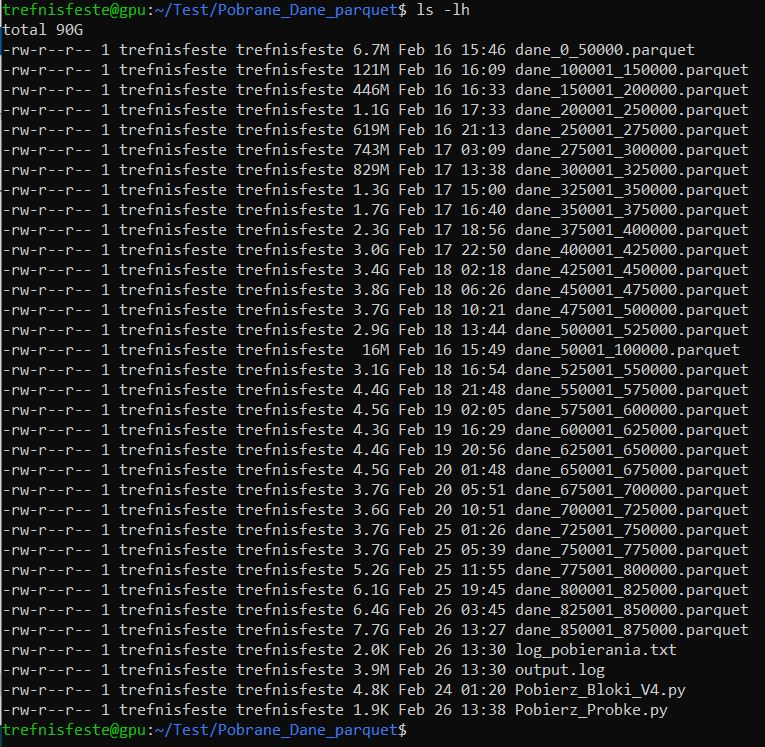
\includegraphics[width=0.95\textwidth]{../screeny/wagi_parquet2.jpg} 
	    \caption{Rozmiar plików w formacie Parquet}
	    \label{fig:rozmiarParquet}
	\end{figure}

	\chapter{Analiza i~prognozowanie opłat transakcyjnych sieci Bitcoin}
	\hspace*{\parindent}W ninejszym rozdziale skupiono sie na analize danych pochodzących z blockchaina Bitcoin. Aby umożliwić dokładne badania przy ograniczonych zasobach obliczeniowych, zdecydowano się na pracę na reprezentatywnej próbcę 1\% danych z każdego przedziału bloków, rozłożonych równomiernie od stycznia 2009 do grudnia 2024. 		Takie podejście pozwala na zachowanie kluczowych cech i~trendów całego zbioru przy jednoczesnym zmniejszeniu jego rozmiaru do 1.6GB. Choć próbka obejmowała 1\% danych z pełnego zbioru, jej rzeczywisty rozmiar (1.6GB) okazał się większy niż proporcjonalnie oczekiwane 0.9GB. Różnica ta wynika ze specyfiki struktury danych, zastosowanego formatu zapisu Parquet oraz zmiennej liczby i~złożoności w poszczególnych okresach historycznych.

	\section{Plan projektu}

	\hspace*{\parindent}Na podstawie tej próbki przeprowadzono szczegółową eksploracyjną analizę danych (EDA), której celem było zidentyfikowanie istotnych zależności oraz wzorców występujących w analizowanych cechach transakcji w sieci Bitcoin. W ramach analizy rozważono między innymi wpływ zmniejszającej się nagrody blokowej na wysokość opłat transakcyjnych oraz zależności  pomiędzy ceną bitcoina a poziomem tych opłat. Do przedstawienia wyników wykorzystano różnorodne techniki wizualizacyjne, umożliwiające ich przejrzystą i~czytelną prezentację.

	Ostatecznym celem pracy było stworzenie modelu predykcyjnego, który na podstawie zidentyfikowanych trendów i~zależności będzie mógł prognozować przyszłe opłaty transakcyjne. Taki model może stanowić cenne narzędzie do analizy dynamiki sieci Bitcoina.

	Zbiór danych zawiera następujące kolumny:
	\begin{itemize}
	    \item \textbf{block\_hash}: Unikalny identyfikator bloku, czyli skrót kryptograficzny, który jednoznacznie określa dany blok w łańcuchu.
	    \item \textbf{block\_height}: Kolejny numer bloku w łańcuchu – im wyższa wartość, tym później blok został dodany do blockchaina.
	    \item \textbf{timestamp}: Znacznik czasu wskazujący, kiedy blok został utworzony (w formacie UNIX, czyli liczba sekund od 1 stycznia 1970).
	    \item \textbf{miner\_reward}: Nagroda przyznana górnikowi za wydobycie bloku – obejmuje nowo wygenerowane bitcoiny (bez opłat transakcyjnych).
	    \item \textbf{txid}: Unikalny identyfikator transakcji, który pozwala odróżnić poszczególne operacje w bloku.
	    \item \textbf{input\_value}: Łączna wartość środków, które zostały wykorzystane jako wejścia w transakcji.
	    \item \textbf{output\_value}: Łączna wartość środków, które zostały przekazane jako wyjścia w transakcji.
	    \item \textbf{fee}: Opłata transakcyjna, stanowiąca różnicę między sumą wartości wejść a sumą wartości wyjść (dla transakcji coinbase zazwyczaj wynosi 0).
	    \item \textbf{size}: Rozmiar bloku lub transakcji wyrażony w bajtach.
	    \item \textbf{weight}: Waga transakcji, określona zgodnie z zasadami obliczania wagi w sieci Bitcoin (wyrażana w jednostkach wirtualnych bajtów, vB).
	\end{itemize}

	\section{Eksploracyjna analiza danych (EDA) i~wizualizacja}
	\hspace*{\parindent}Zbiór danych użyty w niniejszym opracowaniu składa się z 11 325 203 wierszy i~10 kolumn, obejmujących okres od 12 stycznia 2009 r. \textit{(Timestamp('2009-01-12 08:10:44'))} do 16 grudnia 2024 r. \textit{(Timestamp('2024-12-16 12:23:18'))}. Daty zostały przekształcone z formatu UNIX przez konwersję kolumny timestamp do formatu datetime.

	Dodatkowo, korzystając z platformy \textit{https://www.blockchain.com/}\footnote{https://www.blockchain.com/explorer/charts/market-price}, w dniu 18 lutego 2025 roku pobrano plik JSON zawierający historyczne dane cenowe Bitcoina. Stanowią one cenne uzupełnienie zbioru danych, umożliwiając porównanie zmian cenowych z innymi parametrami 			blockchaina. Uwzględnienie danych cenowych przyczyni się do lepszego zrozumienia dynamiki ekosystemu Bitcoina.

	\begin{figure}[H]
	    \centering
	    \includegraphics[width=0.95\textwidth]{../VSC\_screeny/cena\_btc.png} 
	    \caption{Cena bitcoina na przestrzeni lat}
	    \label{fig:cenaBTC}
	\end{figure}

	\begin{figure}[H]
	    \centering
	    \includegraphics[width=0.95\textwidth]{../VSC\_screeny/cena\_btc\_log.png} 
	    \caption{Cena bitcoina na przestrzeni lat (skala logarytmiczna)}
	    \label{fig:cenaBTClog}
	\end{figure}

	Wykres historycznej ceny bitcoina przedstawia zmienność wartości wyrażoną w dolarach amerykańskich tej kryptowaluty w okresie od początku 2009 roku do lutego 2025 roku (\figurename~\ref{fig:cenaBTC}, \figurename~\ref{fig:cenaBTClog}). Pozwala na obserwację długoterminowego trendu cenowego, od początkowo niskich wartości, przez gwałtowne wzrosty, aż do okresów spadków i~konsolidacji.

Wzrost liczby bloków w sieci Bitcoin jest jednym z najbardziej charakterystycznych wskaźników jej ewolucji. Od 2009 roku, kiedy blockchain został uruchomiony, liczba bloków rośnie liniowo wraz z upływem czasu, co w pewnym stopniu odzwierciedla rozszerzanie się łańcucha bloków (\figurename~\ref{fig:blokiBTC}). Należy jednak zauważyc, że ten liniowy wzrost wynika bezpośrednio z konstrukcji sieci, a nie z poziomu jej popularności czy aktywności użytkowników. W związku z tym wykres ten nie dostarcza bezpośrednich informacji o~liczbie transakcji ani o intensywności korzystania z sieci. Pomimo tego, wizualizacja stanowi istotny kontekst dla dalszych analiz dotyczących dynamiki sieci, takich jak zmiany w opłatach transakcyjnych, nagrodach za blok czy momentach halvingu, ponieważ stale rosnący rozmiar blockchaina może mieć wpływ na kwestie skalowalności, czasu potwierdzenia oraz kosztów transakcyjnych.

	\begin{figure}[H]
	    \centering
	    \includegraphics[width=0.95\textwidth]{../VSC\_screeny/bloki\_btc.png} 
	    \caption{Całkowita liczba bloków Bitcoin}
	    \label{fig:blokiBTC}
	\end{figure}

	Nagroda blokowa jest mechanizmem, który w sposób kontrolowany ogranicza podaż nowo tworzonych bitcoinów. Początkowo w 2009 roku, górnicy otrzymywali 50 BTC za każdy wydobyty blok. Jednak co 210 000 bloków (mniej więcej co cztery lata) następuje tzw. halving, czyli nagroda ta jest zmniejszana o połowę. Oznacza to, że do obiegu trafia coraz mniej nowych bitcoinów. W efekcie nowa podaż maleje, podczas gdy popyt np. ze strony inwestorów indywidualnych, instytucji czy funduszy ETF może rosnąć. Taka struktura podaży sprawia, że Bitcoin zyskuje deflacyjny charakter, co może wpływać na wzrost jego wartości w długim terminie.

	Pierwszy halving miał miejsce w 2012 roku, kiedy to nagroda za wydobycie bloku zmniejszyła się z 50 BTC do 25 BTC. Do tej pory miało miejsce 5 halvingów i~obecnie nagroda wynosi 3.125 BTC (\figurename~\ref{fig:halving}). W efekcie, w kolejnych latach widoczny jest wyraźny spadek wysokości nagrody, natomiast rola opłat transakcyjnych wsród górników przypuszczalnie rośnie. W ten sposób sieć Bitcoina utrzymuje swoją stabilność, zgodnie z wizją jej twórcy.

	\begin{figure}[H]
	    \centering
	    \includegraphics[width=0.95\textwidth]{../VSC\_screeny/nagroda\_blokowa.png} 
	    \caption{Zmiana nagrody blokowej w kolejnych halvingach}
	    \label{fig:halving}
	\end{figure}

	Opłaty transakcyjne to dodatkowe wynagrodzenie, które górnicy otrzymują za weryfikację i~dołączenie transakcji do łańcucha bloków. Dla użytkowników średnia opłata w poprzednio zaksięgowanym bloku stanowi wskaźnik obciążenia sieci. W okresach zwiększonego popytu na przetwarzanie transakcji, aby uzyskać szybkie potwierdzenie, użytkownik musi ustawić wyższą opłatę transakcyjną.

	W celach poglądowych wykorzystano wizualizację pochodzącą z otwarto-źródłowego eksploratora mempool.space, który w czasie rzeczywistym prezentuje stan kolejki transakcji w sieci Bitcoin. Narzędzie to umożliwia obserwację prognozowanych rozmiarów kolejnych bloków wraz z odpowiadającymi im przedziałami opłat (wyrażonymi w sat/vB), zalecanych stawek dla różnych poziomów priorytetu, liczby niepotwierdzonych transakcji, wykorzystania pamięci oraz średniego czasu generowania bloków. Chociaż dane z tego serwisu\footnote{https://mempool.space/pl/} nie zostały bezpośrednio uwzględnione w analizie empirycznej, pełni on istotną funkcję pomocniczą – wspierając interpretację zjawisk obserwowanych w sieci oraz ułatwiając zrozumienie mechanizmów kształtowania się opłat transakcyjnych.
	\begin{figure}[H]
	    \centering
	    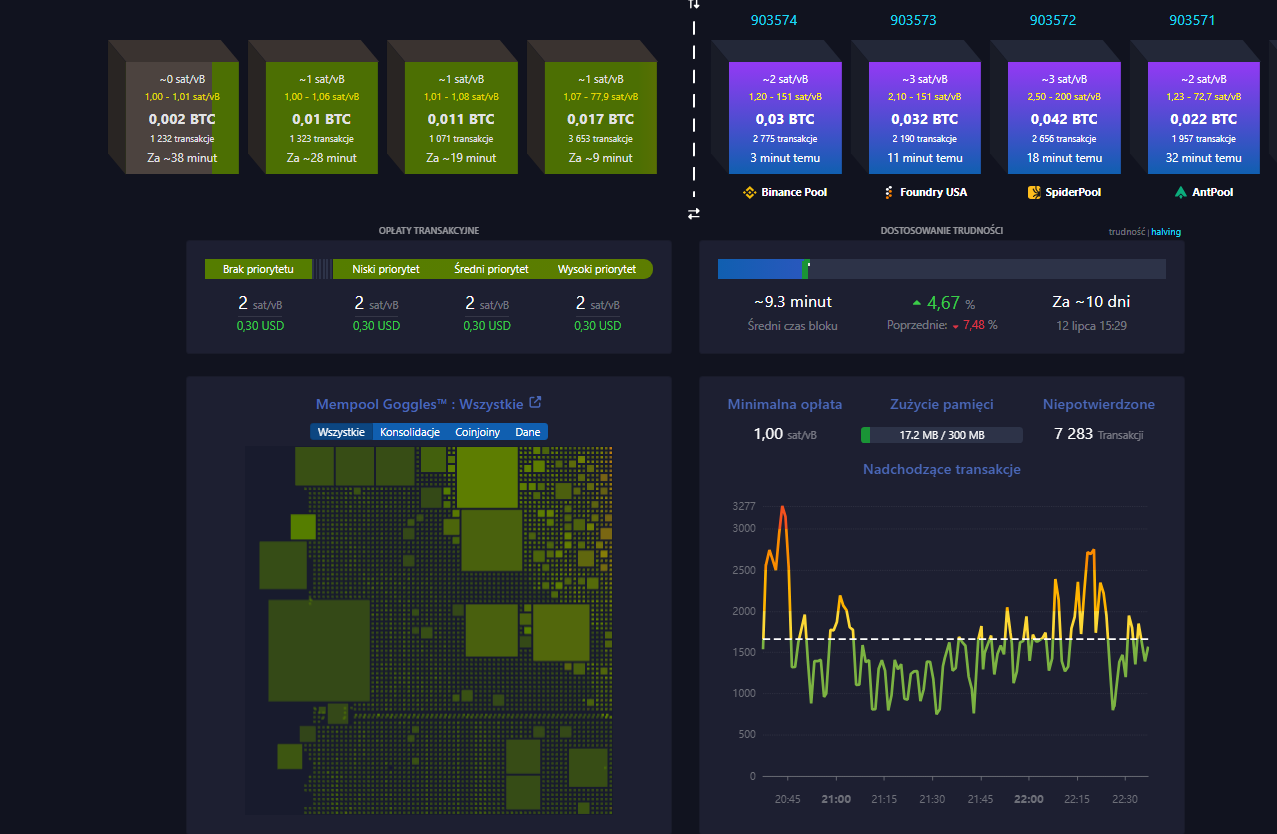
\includegraphics[width=0.8\textwidth]{../screeny/mempoolStrona.png} 
	    \caption{Wizualizacja mempoolu w sieci Bitcoin}
	    \label{fig:mempoolStrona}
	\end{figure}
Główny panel serwisu mempool.space (\figurename~\ref{fig:mempoolStrona}) przedstawia nadchodzące bloki wraz z rozkładem opłat, rekomendowane opłaty dla różnych poziomów priorytetu, wizualizację struktury mempoolu oraz wykres liczby nadchodzących transakcji w czasie.

	\noindent Wykresy przedstawiają średnią opłatę transakcyjną (tygodniową) w dwóch różnych jednostkach:

	\noindent \textbf{Opłata wyrażona w USD.}\\
	\hspace*{\parindent}Opłata pozwala określić, jaki koszt transakcji ponosi użytkownik w dolarach amerykańskich (\figurename~\ref{fig:oplataUSD}). Nawet gdy opłata utrzymuje się na stałym poziomie, zmiany kursu Bitcoina mogą znacząco wpłynąć na ostateczny koszt transakcji wyrażony w~dolarach – wzrost kursu zwiększa jego koszt, a jego spadek obniża.

	\begin{figure}[H]
	    \centering
	    \includegraphics[width=0.95\textwidth]{../VSC\_screeny/oplataUSD\_cenaBTC.png} 
	    \caption{Średnia opłata transakcyjna w USD (tygodniowo) vs. Cena Bitcoina (USD)}
	    \label{fig:oplataUSD}
	\end{figure}

	\noindent \textbf{Opłata wyrażona w satoshi.}\\
	\hspace*{\parindent}Satoshi (najmniejsza jednostka Bitcoina, gdzie 1 BTC = 100 000 000 satoshi) średnio przeznacza się na opłatę. Jest to bardziej bezpośredni wskaźnik obciążenia sieci – niezależny od bieżącego kursu waluty na rynku (\figurename~\ref{fig:oplataSatoshi}). 
	
	\begin{figure}[H]
	    \centering
	    \includegraphics[width=0.95\textwidth]{../VSC\_screeny/oplataSatoshi\_cenaBTC.png} 
	    \caption{Średnia opłata transakcyjna w satoshi (tygodniowo) vs. Cena Bitcoina (USD)}
	    \label{fig:oplataSatoshi}
	\end{figure}

	Zestawienie dwóch perspektyw zapewnia pełniejszy obraz kosztów transakcji w sieci Bitcoin, pozwalając zarówno na analizę wpływu kursu BTC na opłaty, jak i~na śledzenie bezwzględnej ilości bitcoinów przeznaczonych na pokrycie kosztów przetwarzanej transakcji.

	Macierz korelacji przedstawia współczynniki korelacji między parami zmiennych liczbowych w zbiorze danych, co umożliwia szybkie zidentyfikowanie zależności (\figurename~\ref{fig:macierzKorelacji}). Wartości te mieszczą się w przedziale od -1 do 1. Dodatni współczynnik wskazuje na korelację dodatnią (wzrost jednej zmniennej towarzyszy wzrostowi drugiej), ujemny współczynnik oznacza korelację ujemną (gdy jedna zmienna rośnie, druga maleje), a wartości zbliżone do zera sugerują brak istotnej zależności.

	\begin{figure}[H]
	    \centering
	    \includegraphics[width=0.95\textwidth]{../VSC\_screeny/macierz\_korealacji.png} 
	    \caption{Macierz korelacji}
	    \label{fig:macierzKorelacji}
	\end{figure}
	
	Na podstawie macierzy korelacji przedstawionej na rysunku można wskazać kilka zależności pomiędzy analizowanymi zmiennymi:
	\begin{itemize}
	    \item \textbf{Silna dodatnia korelacja pomiędzy \texttt{block\_height} a \texttt{timestamp} ($\rho \approx 1$)} wynika bezpośrednio z architektury łańcucha bloków – każdy kolejny blok jest dodawany w czasie po poprzednim. Zmienna \texttt{timestamp} przyjmuje zatem wartości rosnące wraz ze wzrostem \texttt{block\_height}, co skutkuje niemal idealną liniową zależnością.
	   \item \textbf{Silna dodatnia korelacja pomiędzy \texttt{input\_value} a \texttt{output\_value} ($\rho \approx 1$)} jest naturalna i~wynika z faktu, że różnica między tymi wartościami to właśnie opłata transakcyjna. Ponieważ opłaty stanowią zwykle bardzo niewielki ułamek wartości transakcji (rzędu kilku satoshi na bajt), wartości wejściowe i~wyjściowe są niemal identyczne.
    	  \item \textbf{Zmienna \texttt{size} wykazuje silną korelację z \texttt{weight} ($\rho \approx 0.91$)} co wynika z~konstrukcji danych bloków. Zmienna \texttt{weight} została wprowadzona wraz z aktualizacją SegWit w celu bardziej precyzyjnego odwzorowania kosztów zapisu danych w bloku. Mimo że obie zmienne mierzą „rozmiar” bloku, ich jednostki są różne – jednak rosną razem w bardzo podobny sposób, co skutkuje wysoką korelacją.
   	   \item \textbf{Silna ujemna korelacja pomiędzy \texttt{block\_height} a \texttt{miner\_reward} ($\rho \approx -0.88$)} odzwierciedla mechanizm halvingu zaimplementowany w protokole Bitcoina. Co około 210000 bloków (czyli mniej więcej co 4 lata) nagroda dla górników za wydobycie nowego bloku ulega zmniejszeniu o połowę. W efekcie, im wyższy numer bloku, tym niższa nagroda bazowa przypadająca na daną jednostkę, co skutkuje obserwowanym trendem spadkowym.
	    \item Pozostałe zmienne, takie jak fee, size czy weight, wskazują raczej na słabe korelacje z większością zmiennych cech.
	\end{itemize}

	W celu zbadania siły i~kierunku monotonicznych zależności pomiędzy zmienną objaśnianą (fee), a pozostałymi zmiennymi liczbowymi w zbiorze danych, przeprowadzono analizę korelacji rang Spearmana, która pozwala wykryć również nieliniowe, lecz monotoniczne związki pomiędzy zmiennymi.

	\begin{figure}[H]
	    \centering
	    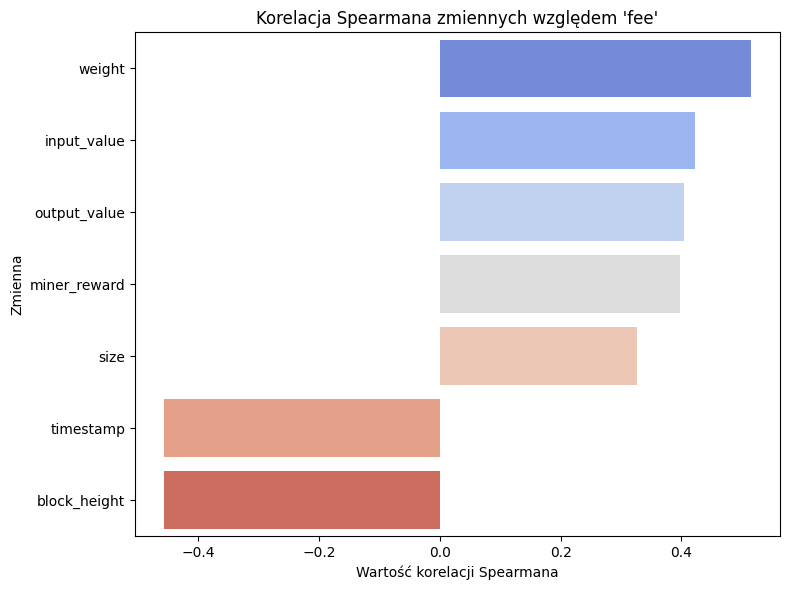
\includegraphics[width=0.95\textwidth]{../VSC\_screeny/Spearmana.png} 
	    \caption{Współczynnik korelacji rang Spearmana}
	    \label{fig:Spearmana}
	\end{figure}

Wyniki analizy korelacji rang Spearmana (\figurename~\ref{fig:Spearmana}) wykazały obecność zarówno dodatnich, jak i~ujemnych zależności pomiędzy wysokością opłaty transakcyjnej a~wybranymi zmiennymi liczbowymi. 
\begin{itemize}
    \item \textbf{Dodatnia korelacja z wagą transakcji (\texttt{weight})} sugeruje, że transakcje o~większym rozmiarze logicznym są częściej powiązane z wyższymi opłatami. Może to wynikać z faktu, że transakcje o większym rozmiarze zajmują więcej przestrzeni w~bloku, a~użytkownicy są skłonni płacić więcej, aby ich transakcja została szybciej przetworzona.
    \item \textbf{Dodatnia korelacja z wartością wejściową i~wyjściową (\texttt{input\_value}, \texttt{output\_value})} może wskazywać, że użytkownicy realizujący transakcje o~większych nominałach są skłonni ustalać wyższe opłaty transakcyjne. Dla osób przesyłających znaczną wartość (np. równowartość tysięcy dolarów), kilka tysięcy satoshi stanowi relatywnie niewielki koszt, a zależy im na szybkim włączeniu transakcji do łańcucha bloków bez długiego oczekiwania.
    \item \textbf{Dodatnia korelacja z nagrodą dla górnika (\texttt{miner\_reward})} może być pochodną zmian w czasie. W początkowym okresie funkcjonowania Bitcoina nagrody blokowe były wysokie (50 BTC). Przy niskim kursie BTC/USD opłaty transakcyjne również stanowiły znaczącą część przychodu górników. Wraz z kolejnymi halvingami i wzrostem ceny Bitcoina udział opłat w tym przychodzie malał, co może tłumaczyć dodatnią korelację między wysokością nagrody a udziałem opłat w analizowanym zbiorze danych.
    \item \textbf{Ujemna korelacja z czasem (\texttt{timestamp}) oraz numerem bloku (\texttt{block\_hei- ght})} może wskazywać na długoterminowy trend spadku rzeczywistego poziomu opłat. Jest to prawdopodobnie efekt zarówno rosnącej wartości BTC (co powoduje, że użytkownicy mogą oferować niższe opłaty w satoshi, zachowując tę samą wartość w USD), jak i~usprawnień technologicznych (optymalizacja struktur danych), które zwiększyły efektywność przetwarzania transakcji.
\end{itemize}

	\section{Przetwarzanie danych}
	\hspace*{\parindent}Aby możliwe było skuteczne zastosowanie algorytmów uczenia maszynowego, dane muszą zostać odpowiednio oczyszczone i przygotowane. Obejmuje to m.in. wybór najbardziej istotnych cech, normalizację danych liczbowych (przeskalowanie ich do wspólnego zakresu) oraz przekształcenie danych tekstowych (kategorycznych) na formę numeryczną, zrozumiałą dla algorytmu. Dopiero tak przetworzone zbiory wydzielone na części treningową, walidacyjną i~testową pozwalają na rzetelne trenowanie, strojenie i~ocenę różnych algorytmów predykcyjnych. Celem tych działań jest zminimalizowanie szumu, zachowanie kluczowych informacji i~zapewnienie modelom spójnych, jednorodnych wejść. Poniższe podrozdziały opisują kolejne kroki tego procesu, prowadzące od oczyszczenia danych aż do trenowania i~weryfikacji różnych algorytmów.

	\subsection{Imputacja brakujących danych numerycznych}
	\hspace*{\parindent}Jednym z wyzwań podczas pracy z danymi jest radzenie sobie z brakującymi wartościami. Braki danych mogą powstać z różnych powodów – od błędów przy rejestracji informacji, przez problemy techniczne, aż po celowe pominięcia obserwacji odstających. Ich występowanie wpływa nie tylko na jakość analiz, ale także na 				wiarygodność przyszłych modeli predykcyjnych.

	Imputacja brakujących danych numerycznych polega na uzupełnieniu braków w~taki sposób, aby jak najlepiej odzwierciedlić rzeczywisty rozkład zmiennych i~nie wprowadzić zniekształceń w zbiorze danych. Dobór metody od prostych statystycznych, takich jak średnia czy mediana, do bardziej złożonych podejść wykorzystujących modele regresyjne lub 			techniki uczenia maszynowego zależy od charakteru danych i~skali ich braków.  

	\begin{figure}[H]
	    \centering
	    \includegraphics[width=0.4\textwidth]{../VSC\_screeny/braki\_danych.png} 
	    \caption{Braki danych w kolumnach}
	    \label{fig:brakiDanych}
	\end{figure}
	
	Po przeanalizowaniu zbioru danych nie wykryto brakujących wartości w żadnej z~kolumn (\figurename~\ref{fig:brakiDanych}).
	
	\subsection{Inżynieria cech}
	\hspace*{\parindent}Inżynieria cech pozwala nam wyodrębnić dodatkowe znaczące informacje z istniejącego zbioru danych, co może poprawić dokładność i~interpretowalność modeli predykcyjnych. Zdecydowano się na inżynierie cech daty, która miała na celu wydobycie informacji o~potencjalnych wzorcach czasowych, które mogą wpływać na wysokość opłat transakcyjnych. 

	\begin{lstlisting}[language=Python,caption=Ekstrakcja cech daty w procesie inżynierii cech,label=EkstrakcjaCech]
	def add_dateparts(df, col):
	    df['Year'] = df[col].dt.year
	    df['Month'] = df[col].dt.month
	    df['Day'] = df[col].dt.day
	    df['DayOfWeek'] = df[col].dt.dayofweek
	
	add_dateparts(df, 'datetime')
	\end{lstlisting}
	
	W tym kroku zostało wykonane wyodrębnianie części daty - dodanie kolumn reprezentujące rok, miesiąc, dzień oraz dzień tygodnia na podstawie istniejącej kolumny \texttt{datetime} (\lstlistingname~\ref{EkstrakcjaCech}).

	\subsection{Utworzenie zbioru treningowego, walidacyjnego i~testowego}
	Podział danych polega na podziale całości dostępnych danych na trzy odrębne zestawy, z których każdy pełni inna funkcję w procesie budowy i~oceny modelu (\figurename~\ref{fig:wymiaryZbiorow}):
	\begin{itemize}
	    \item Zestaw treningowy: używany do trenowania modelu.
	    \item Zestaw walidacyjny: używany do dostrajania parametrów modelu i~unikania nadmiernego dopasowania.
	    \item Zestaw testowy: używany do oceny ostatecznej wydajności modelu na niewidocznych danych.
	\end{itemize}
	
	Oddzielając te podzbiory, zapewniamy, że wydajność modelu jest oceniana na danych, na których nie został przeszkolony.

	\begin{figure}[H]
	    \centering
	    \includegraphics[width=0.6\textwidth]{../VSC\_screeny/wymiary\_zbiorow.png} 
	    \caption{Wymiary zbiorów danych}
	    \label{fig:wymiaryZbiorow}
	\end{figure}
	\hspace*{\parindent}Podział zbiorów danych został dokonany na podstawie przedziałów czasowych:
	\begin{itemize}
	    \item Zbiór trenignowy zawiera dane od 9 stycznia 2009 roku do 1 stycznia 2022 roku.
	    \item Zbiór walidacyjny obejmuje dane od 1 stycznia 2022 roku do 1 stycznia 2024 roku.
	    \item Zbiór testowy składa się z danych od 1 stycznia 2024 roku do 16 grudnia 2024 roku.
	\end{itemize}

	\subsection{Identyfikacja kolumn wejściowych i~docelowej}
	\hspace*{\parindent}W tym kroku utworzono zmienne do których przypisano kolumny wejściowe oraz kolumnę docelową:
	\begin{itemize}
	    \item Kolumny wejściowe (cechy): zmienne, które model wykorzysta do tworzenia prognoz. Wybieramy jedynie kolumny numeryczne (takie jak int i~float), pomijając kolumny o typach datetime czy object.
	    \item Kolumna docelowa: zmienna, którą chcemy przewidzieć, w tym przypadku opłata transakcyjna (fee).
	\end{itemize}

	Zidentyfikujmy również, które z kolumn są liczbowe, a które kategoryczne. Kolumna DayOfWeek została uznana za kategoryczną, co pozwala na odpowiednie przetwarzanie jej wartości w dalszej części analizy.
	
	\subsection{Skalowanie cech numerycznych}
	\hspace*{\parindent}Kolejną dobrą praktyką jest skalowanie cech numerycznych do niewielkiego zakresu wartości. Skalowanie zapewnia, że żadna konkretna cecha nie ma nieproporcjonalnego wpływu na straty modelu. W projekcie zastosowano MinMaxScaler, aby znormalizować dane liczbowe w zakresie [0, 1].

	\subsection{Kodowanie danych kategorycznych}
	\hspace*{\parindent}Ponieważ modele uczenia maszynowego można trenować tylko z danymi liczbowymi, należy przekonwertować zmienne kategoryczne na liczby. One-hot encoding polega na utworzeniu nowej kolumny binarnej (0/1) dla każdej unikalnej kategorii w kolumnie kategorialnej. W projekcie zastosowano tę metodę do kolumny 			\texttt{DayOfWeek}, aby przedstawić dni tygodnia jako wektory binarne. W wyniku zakodowania danych, liczba kolumn w zbiorach wejściowych zwiększyła się (\figurename~\ref{fig:kodowanieDanychKategorycznych}).
	
	\begin{figure}[H]
	    \centering
	    \includegraphics[width=0.6\textwidth]{../VSC\_screeny/wymiary\_zbiorow\_ohe.png} 
	    \caption{Wymiary zbiorów danych po zakodowaniu danych kategorycznych}
	    \label{fig:kodowanieDanychKategorycznych}
	\end{figure}

	\section{Trenowanie i~ocenianie modeli wielowymiarowych}
	\hspace*{\parindent}Na tym etapie zastosowano kilka algorytmów regresji do naszego przetworzonego zbioru danych. Każdy model jest trenowany na zbiorze treningowym i~oceniany na zbiorze walidacyjnym przy użyciu wskaźników (RMSE i $R^2$). Porównując te modele, możemy zidentyfikować, które podejścia są najbardziej obiecujące.

	Dla lepszego zobrazowania, jak każdy z testowanych algorytmów działa, wygenerowano wykres prezentujący porównanie prognozowanych i~rzeczywistych średnich opłat transakcyjnych na zbiorze walidacyjnym. Wartości zostały zagregowane jako średnie tygodniowe, co pozwala lepiej uchwycić ogólne trendy i~różnice między modelami.

	\subsection{Regresja liniowa (Linear Regression)}
	\hspace*{\parindent} Regresja liniowa, to podstawowy algorytm statystyczny, który służy do przewidywania wartości zmiennej ciągłej na podstawie liniowej relacji między zestawem cech, a~zmienną docelową. Model zakłada, że wynik można opisać równaniem w postaci\footnote{Montgomery, D. C., Peck, E. A., \& Vining, G. G. 			Introduction to Linear Regression Analysis. 5th edition. (2012). Strona 12.}:
	\[
	y = \beta_0 + \beta_1 x_1 + \beta_2 x_2 + \dots + \beta_n x_n + \varepsilon,
	\]
	gdzie: $\beta_0$ to stała (intercept), $\beta_i$ to współczynniki określające wpływ poszczególnych cech $x_i$ na wartość prognozowaną, a $\varepsilon$ reprezentuje składnik losowy, czyli błąd modelu.

	Algorytm dąży do wyznaczenia optymalnych wartości współczynników $\beta_i$ tak, aby zminimalizować różnicę między rzeczywistymi a przewidywanymi wartościami y. Najczęściej stosowaną metodą jest metoda najmniejszych kwadratów. Polega ona na znalezieniu takich wartości $\beta_i$ , dla których suma kwadratów różnic między obserwacjami, a 		prognozowanymi wartościami jest najmniejsza.

	Mimo, że regresja liniowa jest ceniona za swoją prostotę, łatwość interpretacji i~niewielkie wymagania obliczeniowe, posiada pewne istotne ograniczenia. Przede wszystkim model opiera się na założeniu liniowości, co może nie oddawać skomplikowanych, nieliniowych zależnoci występujących w rzeczywistych danych. Dodatkowo, jest ona bardzo wrażliwa na wartości odstające, pojedyńcze, ekstremalne obserwacje mogą znacząco wpłynąć na oszczacowane współczynniki, a tym samym zniekształcić prognozy. Pomimo tych wad, regresja liniowa często stanowi punkt wyjścia do bardziej zaawansowanych analiz.

	Model regresji liniowej został utworzony z wykorzystaniem domyślnych parametrów klasy \texttt{LinearRegression} z biblioteki \texttt{scikit-learn}. Nie zastosowano dodatkowej regularyzacji, a funkcja dopasowania modelu została oparta na metodzie najmniejszych kwadratów.

	By ocenić skuteczność modelu Regresji liniowej, \figurename~\ref{fig:wykresLinearRegression} przedstawia porównanie rzeczywistej i~prognozowanej średniej opłaty transakcyjnej (w satoshi) dla zbioru walidacyjnego w ujęciu tygodniowym.	

	\begin{figure}[H]
	    \centering
	    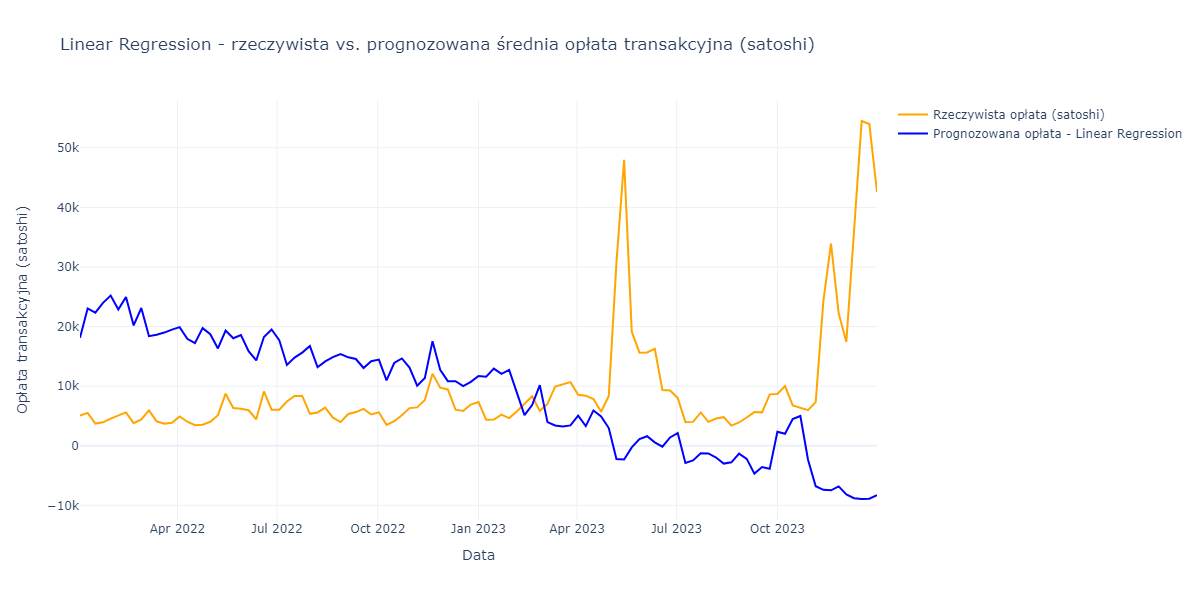
\includegraphics[width=0.95\textwidth]{../VSC\_screeny/ValLinearRegression.png} 
	    \caption{Linear Regression – porównanie opłat}
	    \label{fig:wykresLinearRegression}
	\end{figure}

	\subsection{Regresja grzbietowa (Ridge Regression)}
	\hspace*{\parindent}Regresja grzbietowa, to rozszerzenie regresji liniowej, w której do funkcji kosztu dodaje się składnik karzący duże wartości współczynników. Model minimalizuje sumę kwadratów błędów z dodatkowym współczynnikiem regularizacyjnym\footnote{Cucuringu, M. Lecture 8b: LASSO and Ridge regression. Foundations of 	Data Science. (2019)}:
	\[
	\min_{\beta} \left\{ \sum_{i=1}^{n} \left( y_i - \beta_0 - \sum_{j=1}^{p} \beta_j x_{ij} \right)^2 + \lambda \sum_{j=1}^{p} \beta_j^2 \right\},
	\]
	gdzie $\lambda$ kontroluje siłę karania – im wyższa wartość $\lambda$, tym bardziej model zmniejsza współczynniki, co poprawia jego stabilność, zwłaszcza przy silnej współliniowości między zmiennymi. Regresja grzbietowa pomaga modelowi lepiej radzić sobie z nowymi danymi, zmniejszając zmienność wyników (wariancję). Jednak gdy dane są 			bardzo czyste (mało szumów), może to lekko obniżyć dokładność prognoz.
	
	Model regresji grzbietowej został utworzony z wykorzystaniem klasy \texttt{Ridge} z biblioteki \texttt{scikit-learn}. Przy tworzeniu modelu ustawiono parametr \texttt{random\_state} na wartość 42 w celu zapewnienia powtarzalności wyników. Pozostałe parametry, w tym współczynnik regularyzacji \texttt{alpha}, przyjęły wartości domyślne (\texttt{alpha = 1.0}).	

	Aby lepiej ocenić skuteczność modelu Ridge Regression, \figurename~\ref{fig:wykresRidgeRegression} przedstawia porównanie rzeczywistej i~prognozowanej średniej opłaty transakcyjnej (w satoshi) dla zbioru walidacyjnego w ujęciu tygodniowym.	

	\begin{figure}[H]
	    \centering
	    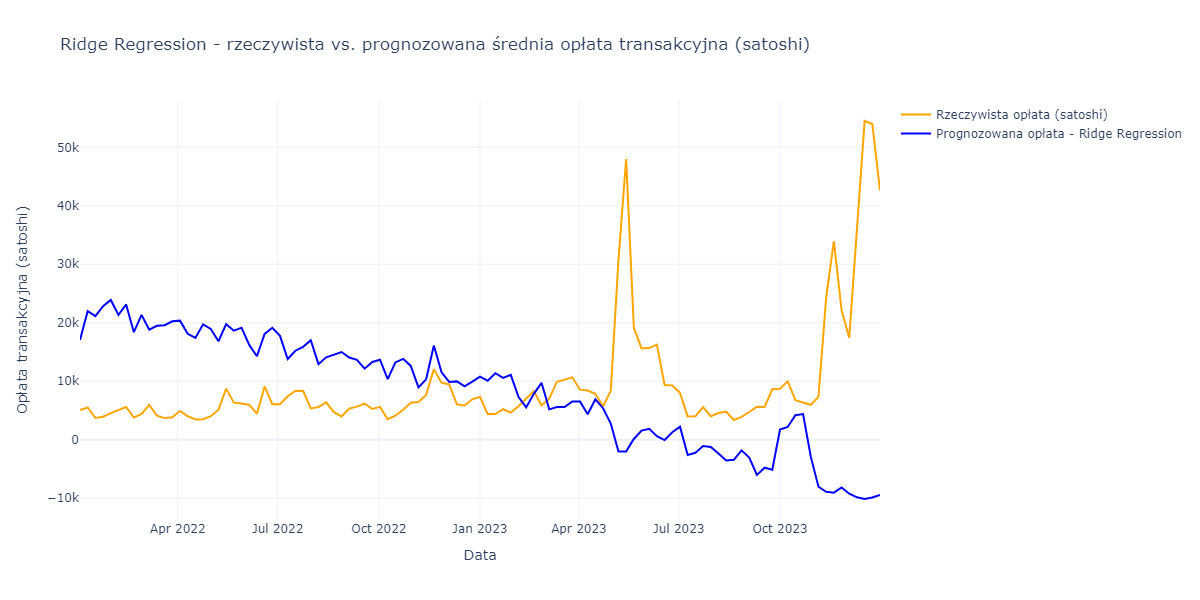
\includegraphics[width=0.95\textwidth]{../VSC\_screeny/ValRidgeRegression.png} 
	    \caption{Ridge Regression – porównanie opłat}
	    \label{fig:wykresRidgeRegression}
	\end{figure}
	
	\subsection{ElasticNet}
	\hspace*{\parindent}ElasticNet to metoda regularizacji, która łączy zalety regresji Lasso (L1) oraz Ridge (L2). Model ElasticNet minimalizuje sumę kwadratów błędów powiększoną o kombinację kar za wartość bezwzględną i~kwadrat współczynników, co zapisuje się równaniem:
	\[
	\min_{\beta} \left\{ \sum_{i=1}^{n}\left(y_i - \beta_0 - \sum_{j=1}^{p}\beta_j x_{ij}\right)^2 + \lambda \left[\alpha \sum_{j=1}^{p} \left|\beta_j\right| + (1-\alpha) \sum_{j=1}^{p} \beta_j^2 \right] \right\},
	\]
	gdzie $\lambda$ to parametr regularyzacji, a $\alpha$ decyduje o udziale kary L1 (Lasso) względem kary L2 (Ridge). Dzięki takiemu podejściu model jest bardziej elastyczny – przy odpowiednim doborze $\alpha$ może zarówno zmniejszać wariancję (poprawiając stabilność i~zdolność modelu do przewidywania nowych danych), jak i~selekcjonować 			zmienne, redukując wpływ nieistotnych cech. ElasticNet sprawdza się szczególnie wtedy, gdy dane charakteryzują się dużą liczbą cech oraz występuje współliniowość między zmiennymi, ponieważ potrafi lepiej radzić sobie z tymi problemami niż pojedyncze metody Lasso czy Ridge.

	Model regresji ElasticNet został utworzony z wykorzystaniem klasy \texttt{ElasticNet} z~biblioteki \texttt{scikit-learn}. Zastosowano domyślne parametry, w tym współczynnik regularyzacji \texttt{alpha = 1.0} (czyli $\lambda$) oraz proporcję kar L1 i~L2 określoną przez \texttt{l1\_ratio = 0.5} (czyli $\alpha$). W celu zapewnienia powtarzalności wyników ustawiono dodatkowo \texttt{random\_state = 42}. Ponieważ model zwracał zawsze tę samą, stałą wartość prognozy, niezależnie od danych wejściowych, co wzbudziło wątpliwości co do poprawności jego działania, autor podjął próbę ręcznego dostosowania parametrów \texttt{alpha} oraz \texttt{l1\_ratio}. Mimo zmiany tych wartości, wynik pozostał niezmienny, co wskazuje na niedopasowanie modelu ElasticNet do specyfiki badanego problemu.

	Aby lepiej ocenić skuteczność modelu ElasticNet, \figurename~\ref{fig:wykresElasticNet} przedstawia porównanie rzeczywistej i~prognozowanej średniej opłaty transakcyjnej (w satoshi) dla zbioru walidacyjnego w ujęciu tygodniowym.	

	\begin{figure}[H]
	    \centering
	    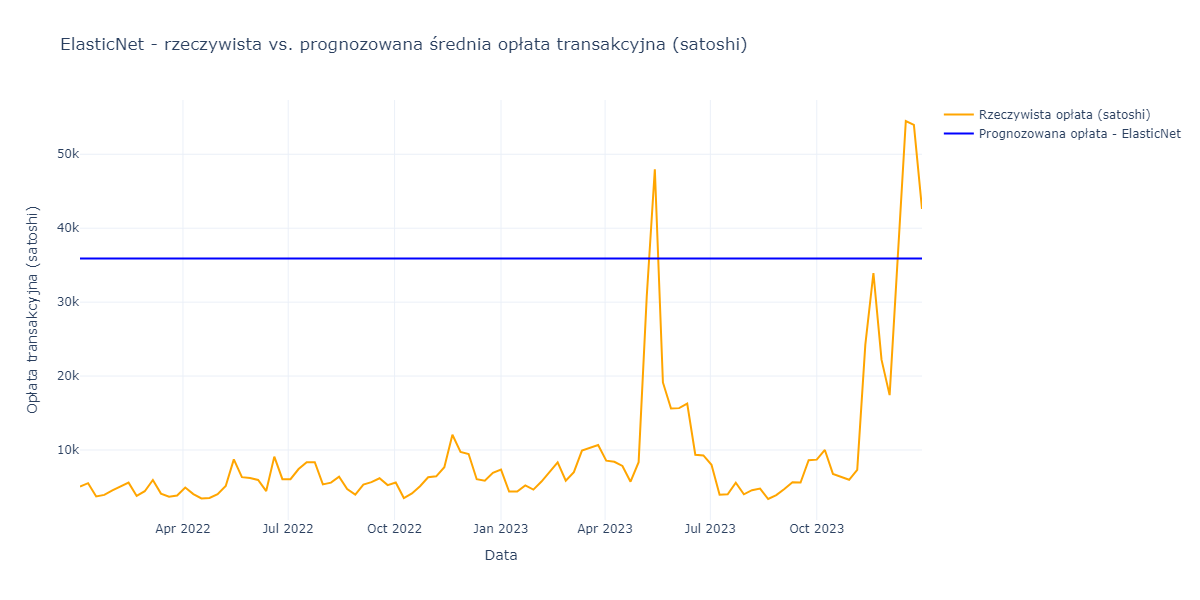
\includegraphics[width=0.95\textwidth]{../VSC\_screeny/ValElasticNet.png} 
	    \caption{ElasticNet – porównanie opłat}
	    \label{fig:wykresElasticNet}
	\end{figure}

	\subsection{Drzewo decyzyjne do regresji (Decision Tree Regressor)}
	Drzewo decyzyjne do regresji, to metoda uczenia maszynowego, która wykorzystuje strukturę drzewa do przewidywania wartości zmiennej ciągłej. Model działa poprzez rekurencyjne dzielenie zbioru danych na mniejsze podzbiory, wybierając przy każdym kroku cechę oraz punkt podziału, które najlepiej rozdzielają dane pod kątem minimalizacji błędu – najczęściej mierzonego jako średni błąd kwadratowy (MSE)\footnote{Baladram, S. Decision Tree Regressor, Explained: A Visual Guide with Code Examples}:
	\[
	MSE = \frac{1}{n} \sum_{i=1}^{n} \left( y_i - \hat{y}_i \right)^2.
	\]
	Podział ten trwa do momentu spełnienia ustalonych kryteriów, takich jak minimalna liczba próbek w liściu czy maksymalna głębokość drzewa. W końcowych węzłach (liściach) przypisuje się prognozowaną wartość, zwykle jako średnią obserwowanych wartości w danym podzbiorze.
	Model ten nie wymaga specjalnej normalizacji danych i~potrafi uchwycić złożone, nieliniowe zależności. Jednakże, może być podatny na przeuczenie, szczególnie gdy drzewo jest zbyt głębokie lub nieprzycięte, co skutkuje zbyt ścisłym dopasowaniem do danych treningowych i~osłabieniem zdolności do generalizacji na nowe dane. Dlatego w praktyce 			często stosuje się techniki ograniczające rozmiar drzewa lub metody zespołowe, takie jak lasy losowe czy gradient boosting, które poprawiają stabilność i~trafność prognoz.

	Model drzewa decyzyjnego został utworzony przy użyciu klasy \texttt{DecisionTreeRegre- ssor} z biblioteki \texttt{scikit-learn}. Ustawiono maksymalną głębokość drzewa na \texttt{max\_dep- th = 10}, aby ograniczyć jego złożoność i~zminimalizować ryzyko przeuczenia. W celu zapewnienia powtarzalności wyników ustawiono również \texttt{random\_state = 42}. Pozostałe parametry przyjęły wartości domyślne.

	Aby lepiej ocenić skuteczność modelu Decision Tree Regressor, \figurename~\ref{fig:wykresDecisionTree} przedstawia porównanie rzeczywistej i~prognozowanej średniej opłaty transakcyjnej (w satoshi) dla zbioru walidacyjnego w ujęciu tygodniowym.	

	\begin{figure}[H]
	    \centering
	    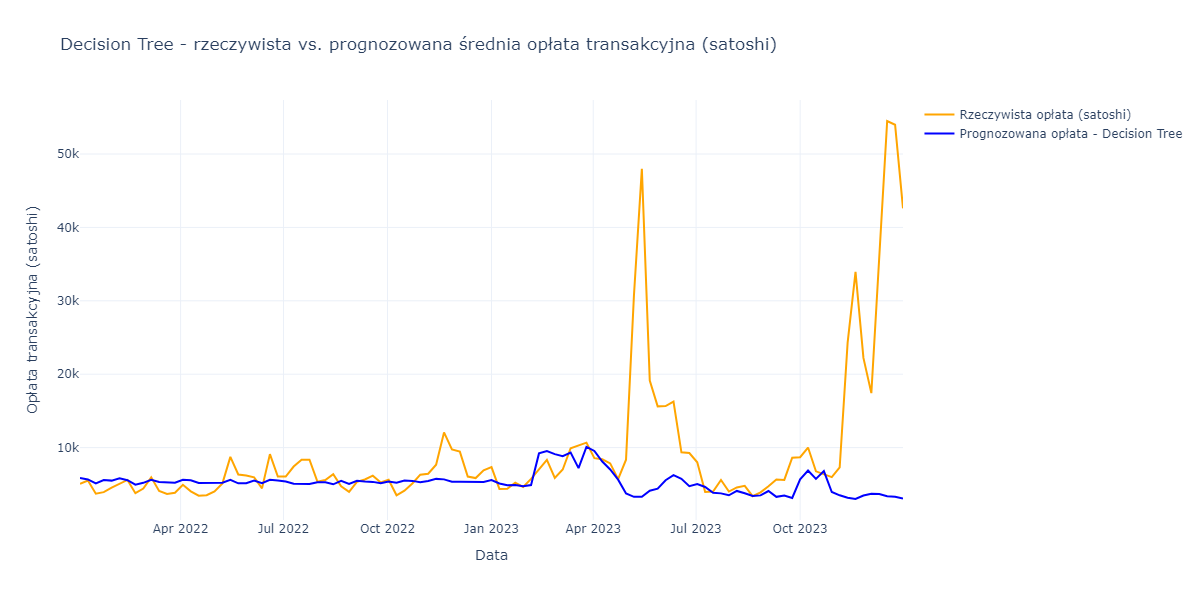
\includegraphics[width=0.95\textwidth]{../VSC\_screeny/ValDecisionTree.png} 
	    \caption{Decision Tree Regressor – porównanie opłat}
	    \label{fig:wykresDecisionTree}
	\end{figure}
	
	\subsection{Las losowy (Random Forest)}
	\hspace*{\parindent}Las losowy to metoda zespołowa oparta na drzewach decyzyjnych, która buduje wiele modeli na losowych podzbiorach danych oraz cech. Każde drzewo w lesie jest trenowane na innej próbce danych (poprzez bootstrap) oraz na losowo wybranej części cech, co wprowadza różnorodność między drzewami. W przypadku regresji 	wynik końcowy uzyskuje się przez uśrednienie prognoz poszczególnych drzew, natomiast dla klasyfikacji stosuje się zasadę głosowania większościowego. Dzięki temu Random Forest jest bardziej odporny na przeuczenie, lepiej generalizuje na nowych danych, a~jednocześnie umożliwia ocenę ważności poszczególnych cech. Metoda ta jest szczególnie 			użyteczna, gdy mamy do czynienia z dużą liczbą cech oraz obserwacji, ponieważ redukuje wariancję i~zwiększa stabilność prognoz w porównaniu do pojedynczych drzew decyzyjnych\footnote{https://www.ibm.com/think/topics/random-forest}.

	Model lasu losowego został utworzony z wykorzystaniem klasy \texttt{RandomForestRegre- ssor} z biblioteki \texttt{scikit-learn}. Ustalono maksymalną głębokość drzew na \texttt{max\_depth = 10} oraz liczbę drzew w lesie na \texttt{n\_estimators = 10}. Parametr \texttt{n\_jobs = -1} pozwolił na równoległe przetwarzanie przy użyciu wszystkich dostępnych rdzeni procesora. W~celu zapewnienia powtarzalności wyników ustawiono \texttt{random\_state = 42}. Pozostałe parametry pozostały bez zmian względem wartości domyślnych.	

	Aby lepiej ocenić skuteczność modelu Random Forest, \figurename~\ref{fig:wykresRandomForest} przedstawia porównanie rzeczywistej i~prognozowanej średniej opłaty transakcyjnej (w satoshi) dla zbioru walidacyjnego w ujęciu tygodniowym.	

	\begin{figure}[H]
	    \centering
	    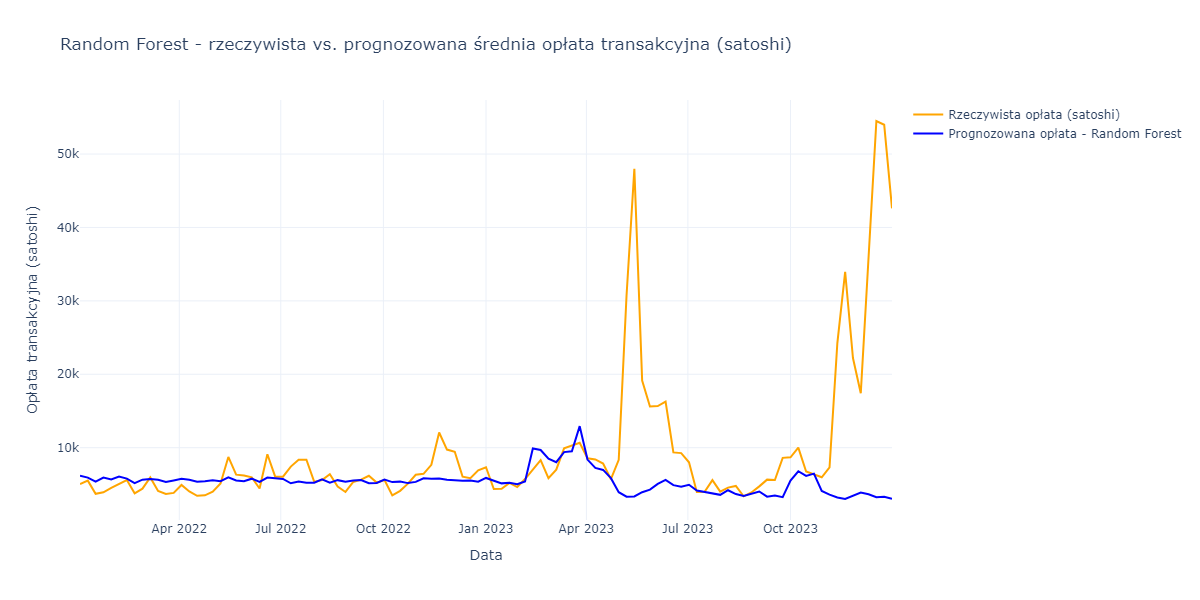
\includegraphics[width=0.95\textwidth]{../VSC\_screeny/ValRandomForest.png} 
	    \caption{Random Forest – porównanie opłat}
	    \label{fig:wykresRandomForest}
	\end{figure}
	
	\subsection{Gradient Boosting}
	\hspace*{\parindent}XGBoost to algorytm oparty na metodzie gradient boosting, który buduje model predykcyjny w sposób iteracyjny, dodając kolejne drzewa decyzyjne, z których każde koryguje błędy poprzednich.

	Podstawowym celem jest minimalizacja funkcji straty, różnicy między rzeczywistymi a przewidywanymi wartościami przez sekwencyjne dodawanie nowych drzew, które uczą się na resztach poprzedniego modelu. W każdej iteracji algorytm oblicza gradienty funkcji straty, a następnie dopasowuje drzewo decyzyjne, które przewiduje te wartości.

	Kluczowym aspektem XGBoost jest włączenie terminu regularizacyjnego do funkcji celu, który nakłada karę za złożoność drzewa i~pomaga zapobiegać przeuczeniu. Dodatkowo, algorytm korzysta z technik subsamplingu zarówno na poziomie obserwacji, jak i~cech, co zwiększa stabilność modelu. Zoptymalizowany pod względem wydajności, XGBoost 			umożliwia równoległe przetwarzanie oraz dynamiczne przycinanie drzew, co czyni go szczególnie efektywnym przy dużych zbiorach danych i~skomplikowanych, nieliniowych zależnościach między zmiennymi\footnote{https://datascience.eu/pl/programowanie-komputerowe/xgboost/}.

	Model XGBoost został utworzony z wykorzystaniem klasy \texttt{XGBRegressor} z biblioteki \texttt{xgboost}. W~celu zapewnienia powtarzalności wyników ustawiono \texttt{random\_state = 42}. Dodatkowo, parametr \texttt{n\_jobs = -1} umożliwił równoległe przetwarzanie na wszystkich dostępnych rdzeniach procesora. Funkcję straty zdefiniowano jako błąd średniokwadratowy poprzez ustawienie \texttt{objective = 'reg:squarederror'}. Pozostałe parametry modelu pozostały na poziomie wartości domyślnych.

	Aby lepiej ocenić skuteczność modelu XGBoost, \figurename~\ref{fig:wykresXGBoost} przedstawia porównanie rzeczywistej i~prognozowanej średniej opłaty transakcyjnej (w satoshi) dla zbioru walidacyjnego w ujęciu tygodniowym.	

	\begin{figure}[H]
	    \centering
	    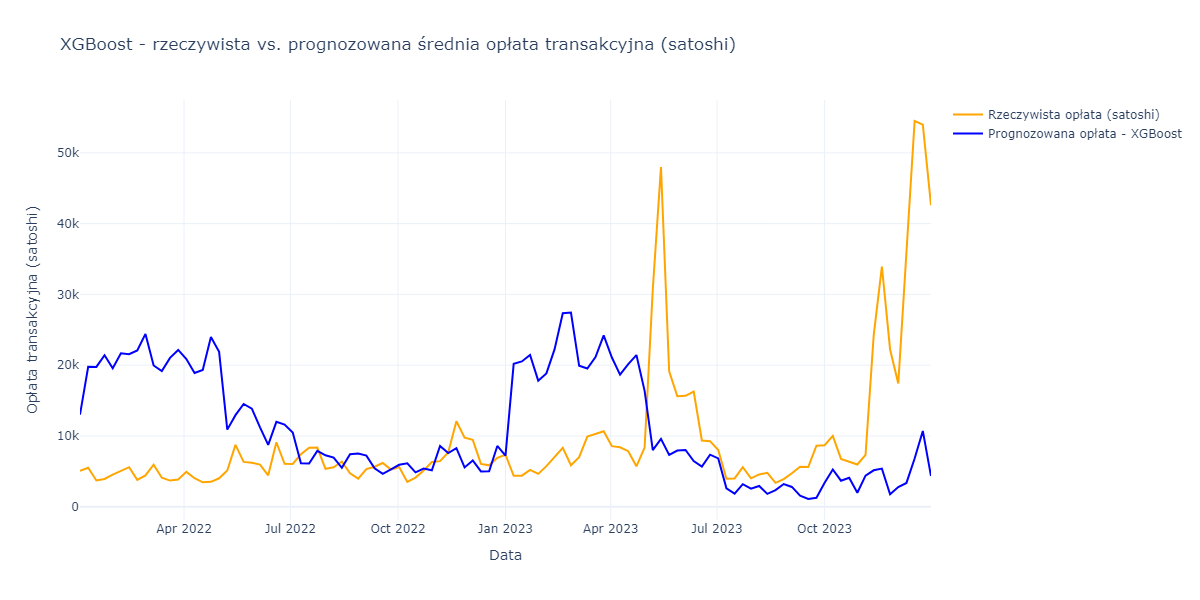
\includegraphics[width=0.95\textwidth]{../VSC\_screeny/ValXGBoost.png} 
	    \caption{XGBoost – porównanie opłat}
	    \label{fig:wykresXGBoost}
	\end{figure}

\subsection{Analiza porównawcza jakości modeli}
\hspace*{\parindent}Po porównaniu różnych modeli zauważono że metody oparte na drzewach decyzyjnych (drzewo decyzyjne, XGBoost) generalnie przewyższają modele regresji liniowej i~ich warianty, szczególnie pod względem RMSE i $R^2$ na zbiorze walidacyjnym (\figurename~\ref{fig:wynikiModeliRegresyjnych}). Decision Tree Regressor i~XGBoost, osiągając najniższe błędy i~najwyższe wyniki $R^2$. Modele te wydają się być solidnym punktem wyjścia do dalszego dostrajania hiperparametrów w celu poprawy jakości przewidywania.

	\begin{figure}[H]
	    \centering
	    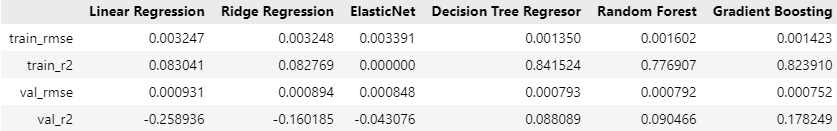
\includegraphics[width=0.95\textwidth]{../VSC\_screeny/modele.png} 
	    \caption{Wyniki modeli regresyjnych}
	    \label{fig:wynikiModeliRegresyjnych}
	\end{figure}
	
	RMSE (Root Mean Squared Error, pierwiastek z średniej kwadratowej błędów) jest miarą dokładności modelu, która informuje, jaka jest średnia wielkość błędu prognoz – im mniejsze RMSE, tym lepiej model przewiduje wartości.

	$R^2$ (współczynnik determinacji) wskazuje, jaka część wariancji zmiennej docelowej jest wyjaśniana przez model. Wartość $R^2$ bliska 1 oznacza, że model bardzo dobrze dopasowuje się do danych, podczas gdy wartość bliska 0 sugeruje, że model nie potrafi efektywnie wyjaśnić zmienności danych.

	\section{Dostrajanie hiperparametrów}
	\hspace*{\parindent}Dostrajanie hiperparametrów ma na celu optymalizację wydajności modelu poprzez identyfikację najlepszej kombinacji hiperparametrów. W tym kroku skupiono się na ulepszeniu modelu XGBoost, który wykazał najlepsze wyniki w poprzednich ocenach. Starannie dostosowując parametry, takie jak wspólczynnik uczenia, liczba 			estymatorów i~głębokość drzewa, dążono do zwiększenia trafności prognoz oraz redukcji błędów na zbiorze walidacyjnym. Poprzez iteracyjne testowanie i~analizę zidentyfikowano optymalną konfigurację parametrów, która pozwala uzyskać najlepsze wyniki predykcyjne.
	
	Poniżej znajdują się podstawowe hiperparametry dla modelu XGBoost, odziedziczone po poprzedniej konfiguracji o najlepszych wynikach (\lstlistingname~\ref{standardParams}). Wraz z kolejnymi testami do słownika dopisywano parametry, które dawały najlepsze rezultaty.
	
	\begin{lstlisting}[language=Python,caption=Słownik standard\_params przed dostrajaniem hiperparametrów ,label=standardParams]
	standard_params = {
	    'random_state': 42,
	    'n_jobs': 1, 
	    'objective': 'reg:squarederror'
	}
	\end{lstlisting}

	W celu dalszej poprawy jakości predykcji modelu XGBoost przeprowadzono iteracyjne dostrajanie hiperparametrów. Podejście to polega na sprawdzaniu różnych wartości kluczowych parametrów i~analizie ich wpływu na błąd (RMSE) zarówno w zbiorze treningowym, jak i~walidacyjnym. Dzięki temu można zidentyfikować konfiguracje, które minimalizują 		przeuczenie (overfitting) oraz zapewniają lepszą zdolność modelu do trafnych prognoz na nowych danych. W dalszej części pracy przedstawiono wyniki dla poszczególnych hiperparametrów, a najlepsze ich wartości zostały włączone do słownika standardowych ustawień modelu XGBoost.

	\begin{figure}[H]
	    \centering
	    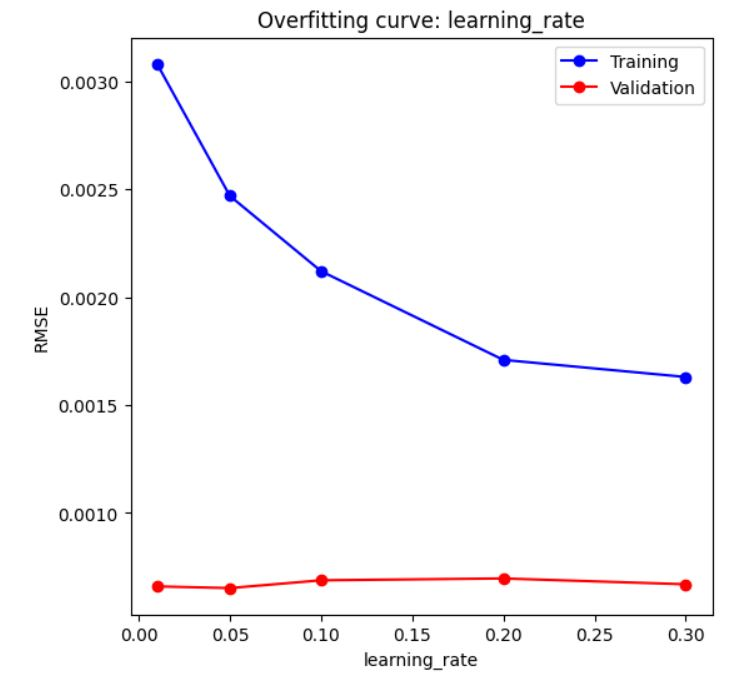
\includegraphics[width=0.55\textwidth]{../VSC\_screeny/learning_rate.JPG} 
	    \caption{Wpływ learning\_rate na błąd RMSE}
	    \label{fig:learningRate}
	\end{figure}
	
	\begin{lstlisting}[language=Python,caption=Dodawanie hiperparametru 'learning\_rate' do słownika standard\_params,label={KodPython3}]
	standard_params['learning_rate'] = 0.1
	\end{lstlisting}

	Wartość parametru \texttt{learning\_rate = 0.1} została wybrana na podstawie analizy krzywej uczenia przedstawionej na \figurename~\ref{fig:learningRate}. Przy tej wartości uzyskano najlepszy kompromis pomiędzy błędem zbioru treningowego i~walidacyjnego. Dalsze zwiększanie współczynnika uczenia nie przynosiło istotnej poprawy na zbiorze walidacyjnym, natomiast zmniejszenie powodowało zwiększenie błędu treningowego bez wyraźnych korzyści w jakości generalizacji.
	
	\begin{figure}[H]
	    \centering
	    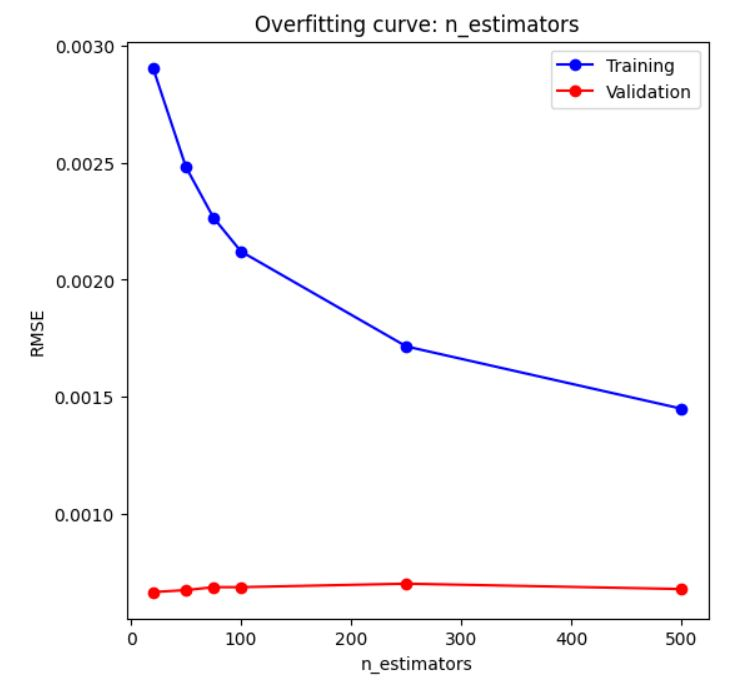
\includegraphics[width=0.55\textwidth]{../VSC\_screeny/n_estimators.JPG} 
	    \caption{Wpływ n\_estimators na błąd RMSE}
	    \label{fig:nEstimators}
	\end{figure}
	
	\begin{lstlisting}[language=Python,caption=Dodawanie hiperparametru 'n\_estimators' do słownika standard\_params,label={KodPython4}]
	standard_params['n_estimators'] = 250
	\end{lstlisting}
	
	Dobór wartości \texttt{n\_estimators = 250} oparto na analizie błędu RMSE w funkcji liczby drzew bazowych, przedstawionej na \figurename~\ref{fig:nEstimators}. Wartość ta zapewniała korzystny kompromis między jakością dopasowania a efektywnością obliczeniową. Dalsze zwiększanie liczby estymatorów przynosiło jedynie niewielką poprawę błędu walidacyjnego, przy jednoczesnym wzroście czasu trenowania modelu.

	
	\begin{figure}[H]
	    \centering
	    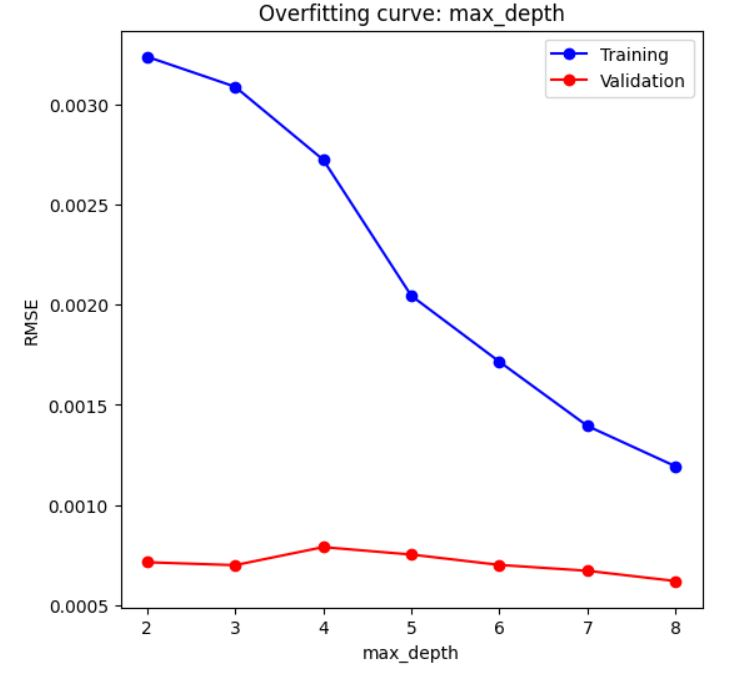
\includegraphics[width=0.55\textwidth]{../VSC\_screeny/max_depth.JPG} 
	    \caption{Wpływ max\_depth na błąd RMSE}
	    \label{fig:maxDepth}
	\end{figure}
	
	\begin{lstlisting}[language=Python,caption=Dodawanie hiperparametru 'max\_depth' do słownika standard\_params,label={KodPython5}]
	standard_params['max_depth'] = 6
	\end{lstlisting}

	Wybór wartości \texttt{max\_depth = 6} został dokonany na podstawie analizy \figurename~\ref{fig:maxDepth}, przedstawiającej wpływ głębokości drzew na błąd RMSE. Głębokość 6 zapewniała najniższy błąd walidacyjny przy jednoczesnym ograniczeniu ryzyka przeuczenia. Dalsze zwiększanie głębokości skutkowało jedynie poprawą dopasowania do zbioru treningowego, bez wyraźnej korzyści dla jakości predykcji na danych walidacyjnych.
	
	\begin{figure}[H]
	    \centering
	    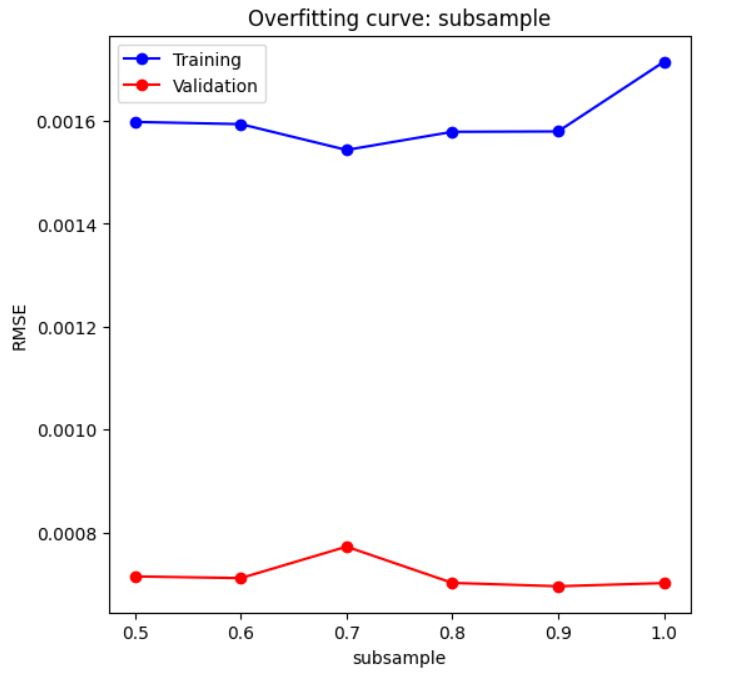
\includegraphics[width=0.55\textwidth]{../VSC\_screeny/subsample.JPG} 
	    \caption{Wpływ subsample na błąd RMSE}
	    \label{fig:subsample}
	\end{figure}
	
	\begin{lstlisting}[language=Python,caption=Dodawanie hiperparametru 'subsample' do słownika standard\_params,label={KodPython6}]
	standard_params['subsample'] = 0.8
	\end{lstlisting}

	Wartość parametru \texttt{subsample = 0.8} została przyjęta na podstawie analizy \figurename~\ref{fig:subsample}, przedstawiającej wpływ proporcji próbkowania na błąd RMSE. Wartości mniejsze niż 1.0 wprowadzają losowość do procesu trenowania, co sprzyja uogólnianiu modelu i~ograniczaniu przeuczenia. Wartość 0.8 zapewniła jeden z najniższych błędów walidacyjnych, przy jednoczesnym zachowaniu stabilności treningu.
	

	Na podstawie przeprowadzonych testów wybrano optymalne hiperparametry (\lstlistingname~\ref{paramsH}).
	
	\begin{lstlisting}[language=Python,caption=Słownik standard\_params po dostrajaniu hiperparametrów,label=paramsH]
	{'random_state': 42,
	 'n_jobs': 1,
	 'objective': 'reg:squarederror',
	 'tree_method': 'gpu_hist',
	 'learning_rate': 0.1,
	 'n_estimators': 250,
	 'max_depth': 6,}
	\end{lstlisting}
	
	\begin{figure}[H]
	    \centering
	    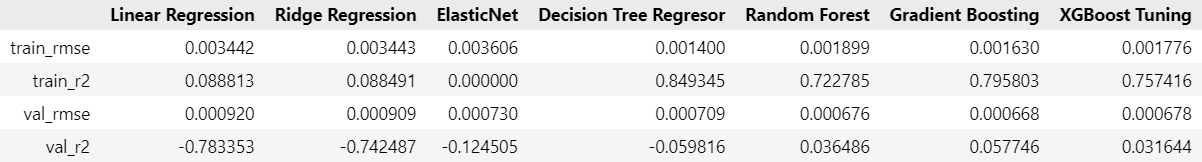
\includegraphics[width=0.95\textwidth]{../VSC\_screeny/modele_po_dostrajaniu.PNG} 
	    \caption{Wyniki modeli regresyjnych po ręcznym dostrajaniu hiperparametrów}
	    \label{fig:wynikiReczneDostrajanie}
	\end{figure}

	Pomimo ręcznego dostrajania hiperparametrów, najnowsze wyniki (XGBoost Tuning) wskazują na nieznaczne pogorszenie jakości prognoz w porównaniu z pierwotną konfiguracją (\figurename~\ref{fig:wynikiReczneDostrajanie}). Może to sugerować, że zmiany parametrów nie zawsze przekładają się na poprawę dopasowania, a niekiedy prowadzą do zjawisk takich jak nadmierne dopasowanie czy zaburzenie procesu uczenia.

	Aby poprawić wyniki modelu, wykorzystano metodę GridSearchCV, która automatycznie przeszukuje siatkę możliwych wartości hiperparametrów, trenując model przy użyciu walidacji krzyżowej dla każdej kombinacji. Dzięki temu możliwe jest znalezienie ustawień, które zapewniają najlepsze rezultaty, choć podejście to może wymagać znacznych 				zasobów obliczeniowych.

	Dla każdej konfiguracji hiperparametrów zdefiniowanej w param\_grid (\lstlistingname~\ref{paramG}) zastosowano 3-krotną walidację krzyżową (cv=3), co pozwala na precyzyjną ocenę modelu XGBoost przy jednoczesnym optymalnym wykorzystaniu zasobów obliczeniowych.
	\begin{lstlisting}[language=Python,caption=Konfiguracja hiperparametrów param\_grid, label=paramG]
	param_grid = {
	    'learning_rate': [0.05, 0.06, 0.07],
	    'n_estimators': [330, 350, 400],
	    'max_depth': [6, 7],
	}
	\end{lstlisting}

	\lstlistingname~\ref{GridSearchCV} przedstawia optymalne hiperparametry uzyskane w procesie GridSearchCV, gdzie dla 18 kombinacji, przy 3-krotnej walidacji (łącznie 54 dopasowania), wyłoniono konfigurację:
	\begin{lstlisting}[language=Python,caption=Wyniki dostrajania hiperparametrów przy użyciu GridSearchCV, label=GridSearchCV]
	Fitting 3 folds for each of 18 candidates, totalling 54 fits
	Best params: {'learning_rate': 0.06, 'max_depth': 6, 'n_estimators': 330}
	Best score: 0.0032048514321261225'
	\end{lstlisting}

	Spośród wszystkich 18 kombinacji hiperparametrów, GridSearchCV wybrał tę, która uzyskała najniższą średnią wartość błędu RMSE w trakcie 3-krotnej walidacji krzyżowej. Oznacza to, że każda konfiguracja była oceniana trzykrotnie - za każdym razem model trenowano na dwóch częściach danych (2/3 zbioru), a testowano na jednej (1/3), przy czym za każdym razem inna część pełniła rolę zbioru walidacyjnego. Wynik końcowy dla danej kombinacji parametrów stanowił średnią z tych trzech pomiarów błędu, co pozwala na bardziej wiarygodną ocenę skuteczności modelu i~ogranicza ryzyko dopasowania do konkretnego podziału danych.

	\begin{figure}[H]
	    \centering
	    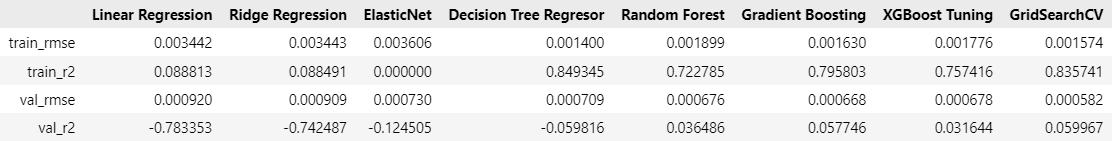
\includegraphics[width=0.95\textwidth]{../VSC\_screeny/modele_gridsearchCV.PNG} 
	    \caption{Wyniki modeli regresyjnych po GridSearchCV}
	    \label{fig:wynikiGridSearchCV}
	\end{figure}
	
	Zastosowanie GridSearchCV przyniosło poprawę w porównaniu z wcześniejszymi modelami. Systematyczne przeszukiwanie przestrzeni hiperparametrów pozwoliło na uzyskanie mniejszego błędu (niższego RMSE) oraz wyższego współczynnika determinacji $R^2$ zarówno na zbiorze treningowym, jak i~walidacyjnym (\figurename~\ref{fig:wynikiGridSearchCV}). Oznacza to, że model jest nie tylko dokładniejszy, ale też lepiej uogólnia się na dane, których nie widział podczas uczenia. W praktyce przekłada się to na bardziej wiarygodne prognozy i~większą stabilność działania modelu.

	\section{Predykcja na zbiorze testowym}
	\hspace*{\parindent}W niniejszym rozdziale dokonano oceny ostatecznej jakości wybranego, najlepszego modelu XGBoost (po dostrajaniu hiperparametrów metodą GridSearchCV) na niezależnym zbiorze testowym. Celem tej analizy było zweryfikowanie, czy wytrenowany model dobrze uogólnia się na dane, których wcześniej nie widział, oraz określenie jego rzeczywistej skuteczności predykcyjnej w praktyce.

Po wybraniu najlepszego modelu (GridSearchCV), kolejnym krokiem jest ocena jego ostatecznej jakości na niezależnym zbiorze testowym. Dzięki temu możemy zweryfikować, czy wytrenowany model dobrze uogólnia się na dane, których wcześniej nie widział.
	\begin{lstlisting}[language=Python,mathescape=true,caption=Wyniki predykcji na zbiorze testowym, label=wyniki]
	Test RMSE: 0.0006495221424186194
	Test $R^2$: 0.2305409589515538
	\end{lstlisting}
	RMSE na poziomie 0.00065 BTC oznacza, że przeciętna różnica między prognozowaną a rzeczywistą opłatą transakcyjną wynosi około 0.00065 BTC, co w przeliczeniu na walutę (np. USD lub PLN) może stanowić znaczącą wartość (\lstlistingname~\ref{wyniki}).

	Umiarkowane $R^2$ oznacza, że model wyjaśnia jedynie około 23\% zmienności obserwowanych danych. Sugeruje to, że model tylko częściowo odzwierciedla zależności w~danych testowych, dlatego wciąż istnieje przestrzeń do poprawy jakości predykcji.

	W celu lepszego zobrazowania skuteczności modelu po strojeniach hiperparametrów, porównano rzeczywistą średnią tygodniową opłatę transakcyjną z wartościami prognozowanymi na zbiorze testowym (\figurename~\ref{fig:PrognozaGridSearchCV}).

	\begin{figure}[H]
	    \centering
	    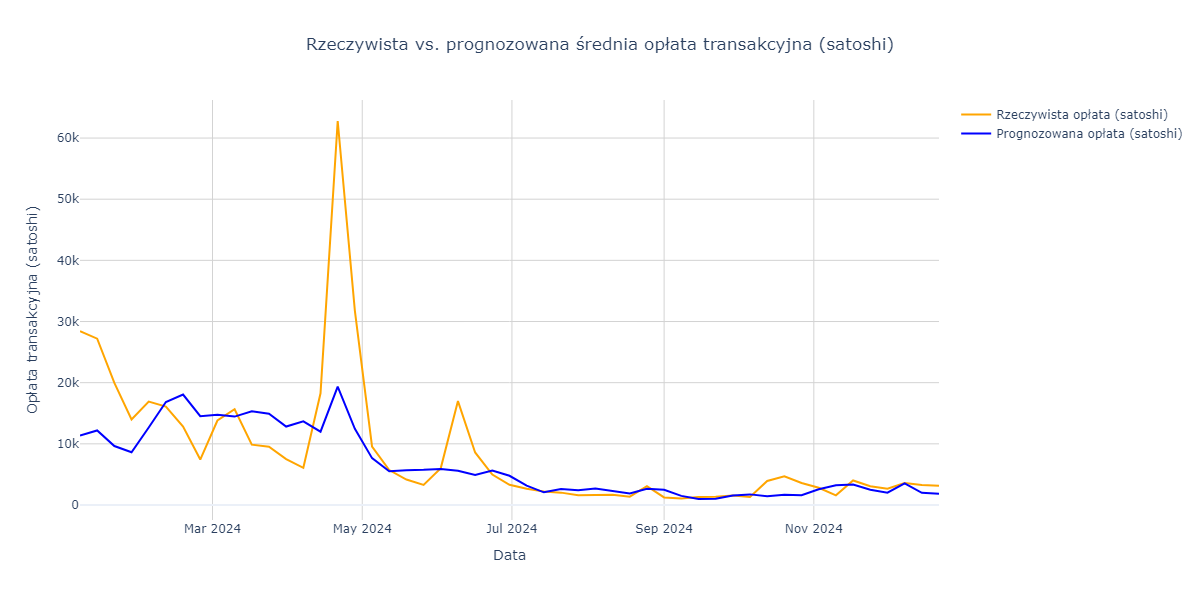
\includegraphics[width=0.95\textwidth]{../VSC\_screeny/PrognozowanieGridSearchCV.png} 
	    \caption{Prognozowana średnia opłata transakcyjna (satoshi)}
	    \label{fig:PrognozaGridSearchCV}
	\end{figure}

	Ogólnie, model, mimo optymalizacji na zbiorach treningowym i~walidacyjnym, wciąż nie osiąga zadowalającej skuteczności na nowych danych. Należy zwrócić uwagę, że największe niedopasowania modelu względem rzeczywistej wartości średnich opłat transakcyjnych jest w okolicach kwietnia 2024, czyli w momencie ostatniego halvingu Bitcoina. Zjawisko to prowadzi do zwiększonej niepewności, zmian zachowań uczestników rynku oraz gwałtownymi zmianami opłat. Model w tym okresie wyraźnie sobie nie radzi, co sugeruje, że metody regresyjne maja trudność z uchwyceniem gwałtownych, nieliniowych zmian podczas halvingów.  

Dodatkowo, w poczatkowych latach istnienia Bitcoina średnie opłaty transakcyjne w satoshi były znacznie wyższe, jednak miały one niewielka wartość w przeliczeniu na waluty (USD/PLN). \enlargethispage{2\baselineskip} Wraz z rosnaca popularnoscia oraz wzrostem kursu Bitcoina, realny koszt opłaty transakcyjnej w dolarach czy złotych nieznaczaco wzrósł. W obecnej analizie model nie uwzględnia dynamicznie rosnacej ceny Bitcoina. Prognozowana opłata na poziomie około  0.00064952 odpowiada 64 952 satoshi, więc znacznie przewyższa typowa opłatę transakcyjna.

	\section{Modele jednowymiarowe}
	\hspace*{\parindent}Po przeprowadzeniu analizy i~oceny modeli wielowymiarowych, w dalszej części pracy zdecydowano się na przetestowanie podejścia jednowymiarowego, w którym do prognozowania wysokości opłaty transakcyjnej wykorzystuje się wyłącznie jedną zmienną wejściową - numer bloku (\textit{block\_height}). Tego rodzaju podejście pozwala ocenić, w jakim stopniu sama struktura czasowa, bez uwzględnienia dodatkowych informacji technicznych dotyczących transakcji, jest wystarczająca do estymacji wartości opłaty.

Zastosowanie modelu jednowymiarowego jest również uzasadnione praktycznie: umo\-żliwia on wygenerowanie prognozy dla konkretnego bloku bez konieczności znajomości szczegółowych danych wejściowych, które w momencie prognozy mogą być jeszcze niedostępne. Ponadto, pozwala to porównać skuteczność prostego modelu bazującego wyłącznie na czasie (reprezentowanym przez rosnący numer bloku) z bardziej złożonymi modelami opartymi na wielu cechach. Analiza ta może również wskazać, czy i~w jakim stopniu opłaty transakcyjne podlegają przewidywalnym trendom czasowym.

\subsection{Model regresji liniowej (Linear Regression)}

Aby uniknąć zakłóceń wynikających z anomalii charakterystycznych dla początkowego etapu funkcjonowania sieci Bitcoin, dane zostały podzielone w następujący sposób:
\begin{itemize}
    \item \textbf{Zbiór treningowy} - od pierwszego halvingu do ostatniego halvingu (listopad 2012 - kwiecień 2024),
    \item \textbf{Zbiór testowy} - od ostatniego halvingu (kwiecień 2024) do grudnia 2024.
\end{itemize}

\begin{lstlisting}[language=Python,caption=Podział danych na zbiory treningowy i testowy,label=ZbioryJ]
	block_halving1 = df[df['datetime'] >= '2012-11-28'].iloc[0]['block_height']
	block_halving4 = df[df['datetime'] >= '2024-04-19'].iloc[0]['block_height']
	
	train_df = df[(df['block_height'] >= block_halving1) & (df['block_height'] < block_halving4)]
	test_df  = df[df['block_height'] >= block_halving4]
\end{lstlisting}

Następnie przeprowadzono normalizację danych. Tak przygotowany zbiór został wykorzystany do trenowania modelu regresji liniowej, którego celem była predykcja wysokości opłat transakcyjnych na podstawie numeru bloku. Model został przeszkolony na zbiorze treningowym, a jego skuteczność oceniono na zbiorze testowym. Rysunek~\ref{fig:WZ} przedstawia wymiary poszczególnych podzbiorów danych, uwzględnionych w dalszej analizie.

	\begin{figure}[H]
	    \centering
	    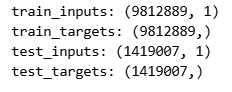
\includegraphics[width=0.55\textwidth]{../VSC\_screeny/Wymiary_zbiorow_jednowymiarowych.png} 
	    \caption{Wymiary zbiorów danych}
	    \label{fig:WZ}
	\end{figure}

W celu oceny skuteczności regresji liniowej w prognozowaniu opłat transakcyjnych na podstawie samego numeru bloku (\textit{block\_height}), dokonano predykcji na zbiorze testowym. Uzyskane wartości zostały następnie przeskalowane do postaci satoshi oraz dolarów amerykańskich (USD), co umożliwiło ocenę modelu w dwóch ujęciach: technicznym i~praktycznym.

	\begin{figure}[H]
	    \centering
	    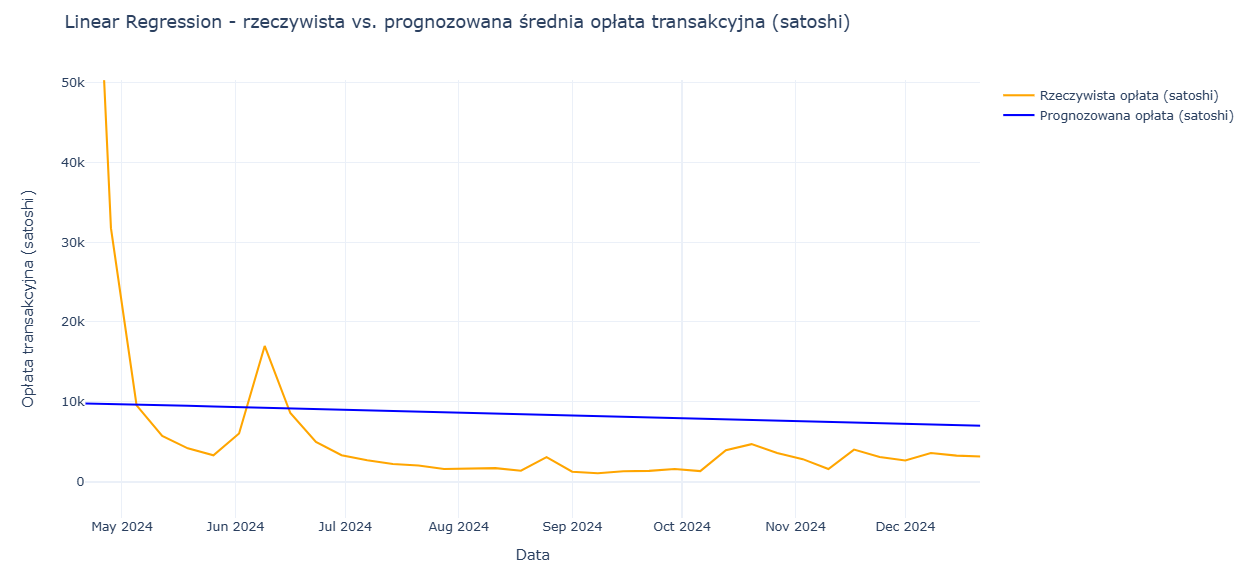
\includegraphics[width=0.95\textwidth]{../VSC\_screeny/JednowymiaroweLiniowaSatoshi.PNG} 
	    \caption{Linear Regression - porównanie opłat (Satoshi)}
	    \label{fig:jednowymiarowyLRSathosi}
	\end{figure}

Na \figurename~\ref{fig:jednowymiarowyLRSathosi} przedstawiono porównanie rzeczywistych oraz prognozowanych wartości średnich tygodniowych opłat transakcyjnych wyrażonych w satoshi. Wykres ten pokazuje, że model regresji liniowej uchwycił jedynie ogólny trend spadkowy, jednak jego predykcje znacząco odbiegają od rzeczywistych wartości - są wyraźnie przeszacowane.

	\begin{figure}[H]
	    \centering
	    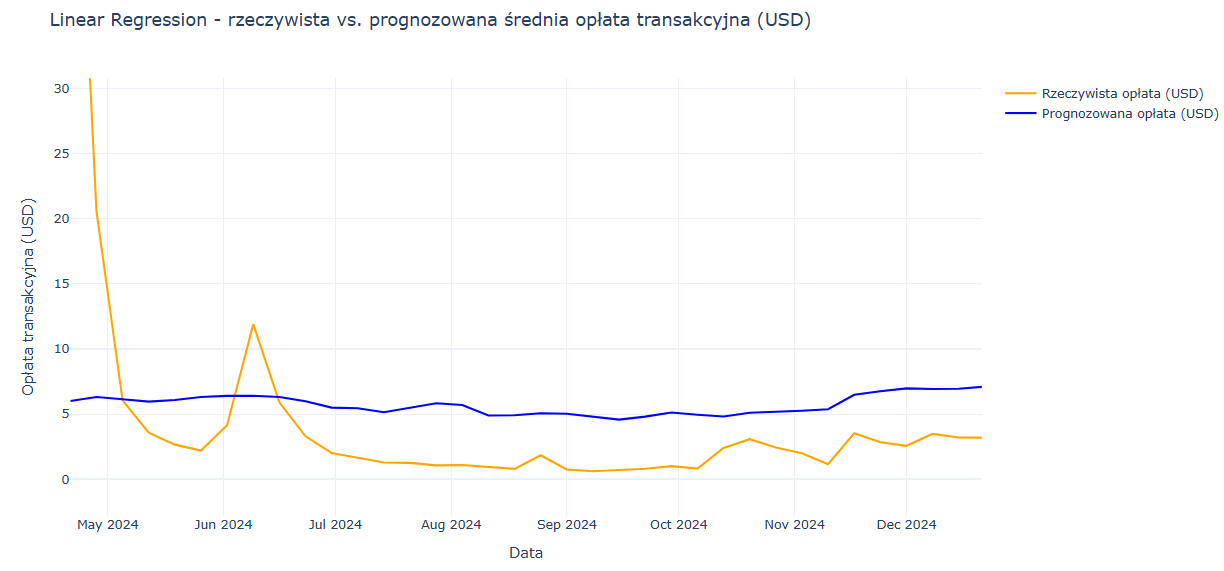
\includegraphics[width=0.95\textwidth]{../VSC\_screeny/JednowymiaroweLiniowaUSD.PNG} 
	    \caption{Linear Regression - porównanie opłat (USD)}
	    \label{fig:jednowymiarowyLRUSD}
	\end{figure}

Z kolei \figurename~\ref{fig:jednowymiarowyLRUSD} przedstawia analogiczne porównanie, lecz w ujęciu wartości w dolarach. Takie podejście pozwala na bardziej intuicyjną interpretację ekonomiczną prognozowanej wysokości opłaty transakcyjnej. Również tutaj widoczne jest systematyczne przeszacowanie przez model.

	\begin{lstlisting}[language=Python,mathescape=true,caption=Wyniki predykcji na zbiorze testowym, label=wynikiJednowymiarowy]
	Test RMSE: 0.0007288125531538861
	Test $R^2$: 0.021213389898962026
	\end{lstlisting}

Uzyskana wartość RMSE oznacza, że przeciętne odchylenie prognozy od wartości rzeczywistej wynosi około 0.00073 BTC (czyli ok. 73 000 satoshi), co jest wartością istotną w praktyce. Wartość współczynnika determinacji  $R^2$ wynosząca jedynie 0.0212 świadczy o bardzo niskim poziomie wyjaśnienia zmienności danych przez model.

Wnioski płynące z analizy są jednoznaczne: model regresji liniowej, mimo że wykazuje pewną czułość na trend spadkowy, nie jest wystarczająco dokładny, aby trafnie odwzorować rzeczywiste zmiany w poziomie opłat transakcyjnych. Może to wynikać z faktu, że numer bloku sam w sobie nie zawiera wystarczającej ilości informacji predykcyjnej. W kolejnej sekcji rozważone zostanie zastosowanie bardziej zaawansowanego podejścia szeregów czasowych z wykorzystaniem modelu SARIMA. Co istotne, mimo ograniczonej dokładności predykcji, model zdołał uchwycić długoterminową tendencję spadku opłat transakcyjnych wyrażonych w BTC, co może być efektem rosnącej wartości Bitcoina oraz coraz większej efektywności mechanizmów przesyłania transakcji w~sieci.

	\subsection{Model szeregów czasowych z uwzględnieniem sezonowości (SARIMA)}
	\hspace*{\parindent}Oprócz klasycznych alogrytmów regresyjnych oraz modeli opartych na drzewach decyzyjnych, zdecydowano się również na zastosowanie modelu szeregów czasowych z uwzględnieniem sezonowości SARIMA (Seasonal Autoregressive Integrated Moving Average).

	Model SARIMA stanowi rozszerzenie klasycznego modelu ARIMA o komponent sezonowy, co umożliwia modelowania i~prognozowanie zjawisk wykazujących powtarzalne wzorce w określonych przedziałach czasowych. Dzięki uwzględnieniu zarówno autokorelacji, jak i~efektów sezonowych, model ten jest szczególnie użyteczny w analizie danych, w których występują cykliczne zmiany jak ma to miejsce w przypadku wybranych aspektów aktywności sieci blockchain, w tym opłat transakcyjnych.

Matematycznie model SARIMA opisywany jest przez zestaw parametrów: (p, d, q) × (P, D, Q, s), gdzie (p, d, q) odpowiadają rzędom części autoregresyjnej, różnicowania i~średniej ruchomej w komponencie niesezonowym, natomiast (P, D, Q, s) odpowiadają analogicznym rzędom oraz długości okresu sezonowego w komponencie sezonowym. 
	
	\begin{figure}[H]
	    \centering
	    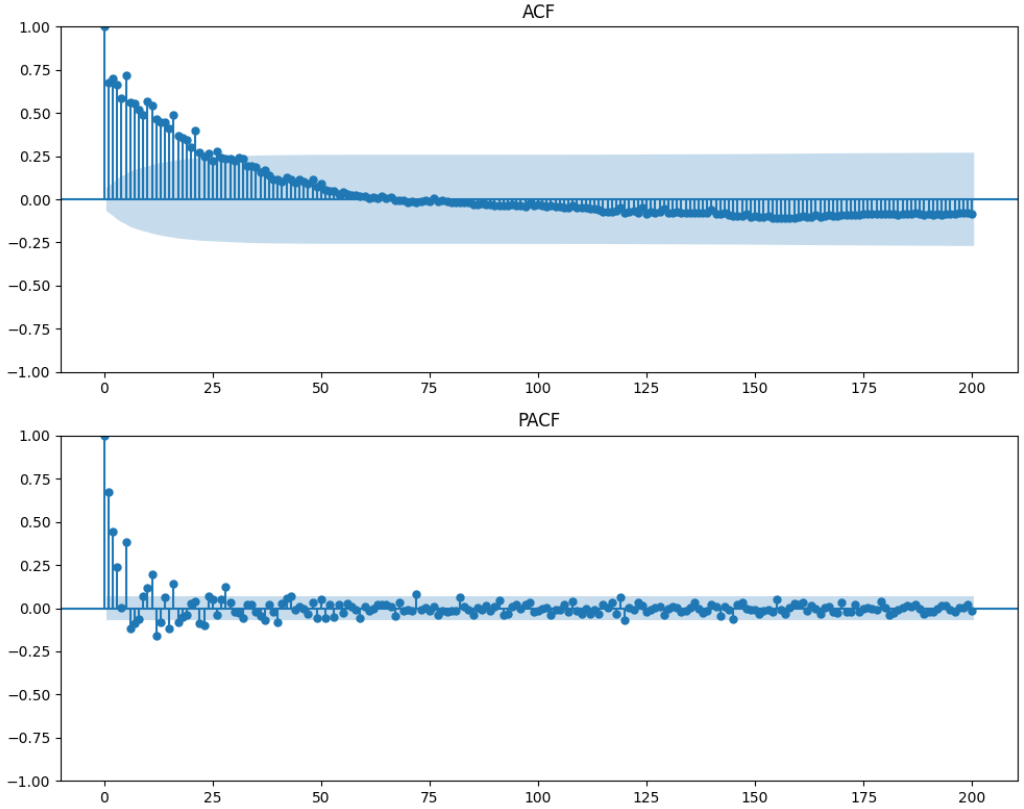
\includegraphics[width=0.95\textwidth]{../VSC\_screeny/ACF_PACF.png} 
	    \caption{Wykresy ACF i PACF}
	    \label{fig:ACFiPACF}
	\end{figure}

	Przed budową modelu SARIMA przeprowadzono analizę wykresów funkcji autokorelacji (ACF) oraz częściowej autokorelacji (PACF) (\figurename~\ref{fig:ACFiPACF}). Wykres PACF wskazuje na istotną korelację dla pierwszego opóźnienia, natomiast wykres ACF charakteryzuje się stopniowym spadkiem wartości, co sugeruje obecność składników autoregresyjnych i~średniej ruchomej. Na podstawie wykresów ACF i PACF przyjęto strukturę (1,1,2) dla części niesezonowej modelu SARIMA. Silny pik na wykresie PACF przy pierwszym opóźnieniu uzasadnia wybór składnika autoregresyjnego rzędu 1, natomiast stopniowo zanikające wartości ACF wskazują na obecność składnika MA rzędu 2. Różnicowanie (d=1) zastosowano ze względu na niestacjonarność szeregu. Okres sezonowości ustalono na 210 okien po 1000 bloków, co odpowiada cyklowi halvingu w sieci Bitcoin (210 000 bloków).  W środowisku kryptowalut panuje powszechne przekonanie, że zdarzenia halvingu wyznaczają kluczowe punkty zwrotne w funkcjonowaniu sieci Bitcoina zarówno w wymiarze ekonomicznym (np. wpływ na podaż i~cenę), jak i~technicznym (np. zmiany zachowań górników i~użytkowników). Zjawisko to może również przekładać się na cykliczne zmiany opłat transakcyjnych. Dlatego przyjęcie długości sezonu odpowiadającej odstępowi między halvingami jest merytorycznie uzasadnione i~może pomóc w uchwyceniu powtarzających się wzorców w analizowanym szeregu czasowym.  Dla części sezonowej przyjęto minimalne wartości parametrów (0,1,1,210), umożliwiające uchwycenie cyklicznych komponentów szeregu.

	Po ustaleniu struktury modelu SARIMA, dokonano jego trenowania na zbiorze treningowym obejmującym okres od pierwszego do ostatniego halvingu Bitcoina (listopad 2012 - kwiecień 2024). Następnie wykonano predykcję na zbiorze testowym, obejmującym dane od ostatniego halvingu (kwiecień 2024) do grudnia 2024. Wyniki uzyskane z~modelu SARIMA przedstawiono na wykresach, porównując rzeczywiste oraz prognozowane wartości opłat transakcyjnych zarówno w satoshi, jak i w dolarach amerykańskich (USD).
	
	Na Rysunku~\ref{fig:SARIMASatoshi} zaprezentowano przebieg prognozy SARIMA w porównaniu do rzeczywistych średnich tygodniowych opłat transakcyjnych wyrażonych w satoshi. Wykres wskazuje, że model zdołał częściowo odwzorować tendencję zmian opłat, jednak w wielu miejscach widoczne są istotne różnice między prognozą a rzeczywistymi wartościami, w tym momenty przeszacowania.
	
	\begin{figure}[H]
	\centering
	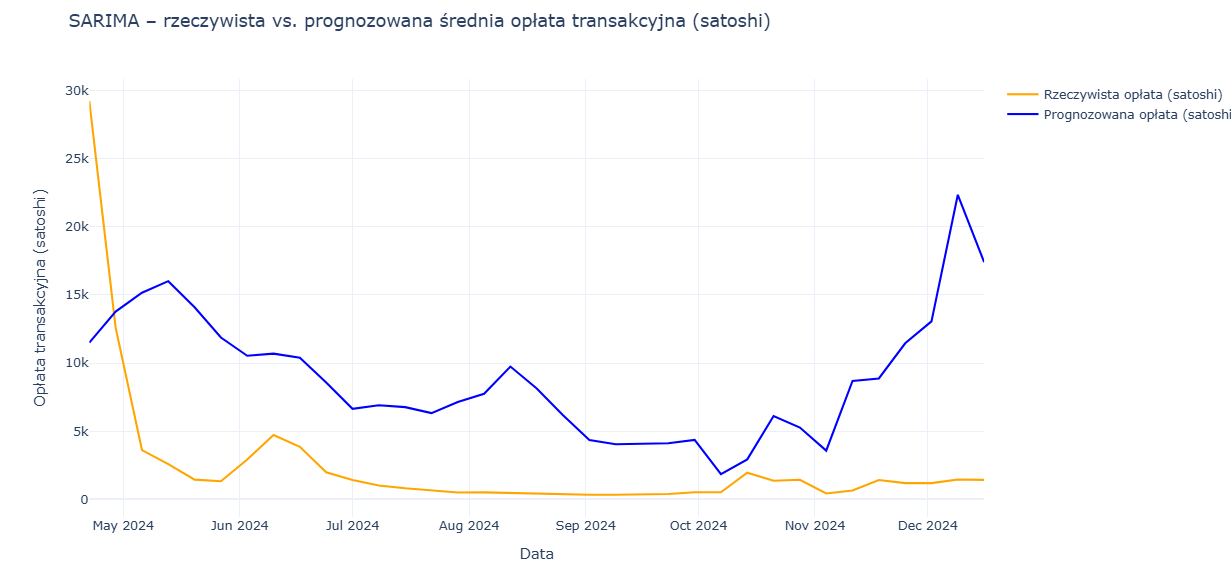
\includegraphics[width=0.95\textwidth]{../VSC_screeny/SARIMA_SATOSHI.PNG}
	\caption{SARIMA – rzeczywista vs. prognozowana opłata transakcyjna (satoshi)}
	\label{fig:SARIMASatoshi}
	\end{figure}
	
	Analogiczne porównanie opłat przedstawione zostało na Rysunku~\ref{fig:SARIMAUSD}, tym razem w jednostkach USD. Podobnie jak w przypadku satoshi, model SARIMA odzwierciedla ogólny kierunek zmian, jednak precyzja predykcji jest ograniczona, co widoczne jest szczególnie w okresach większej zmienności.
	
	\begin{figure}[H]
	\centering
	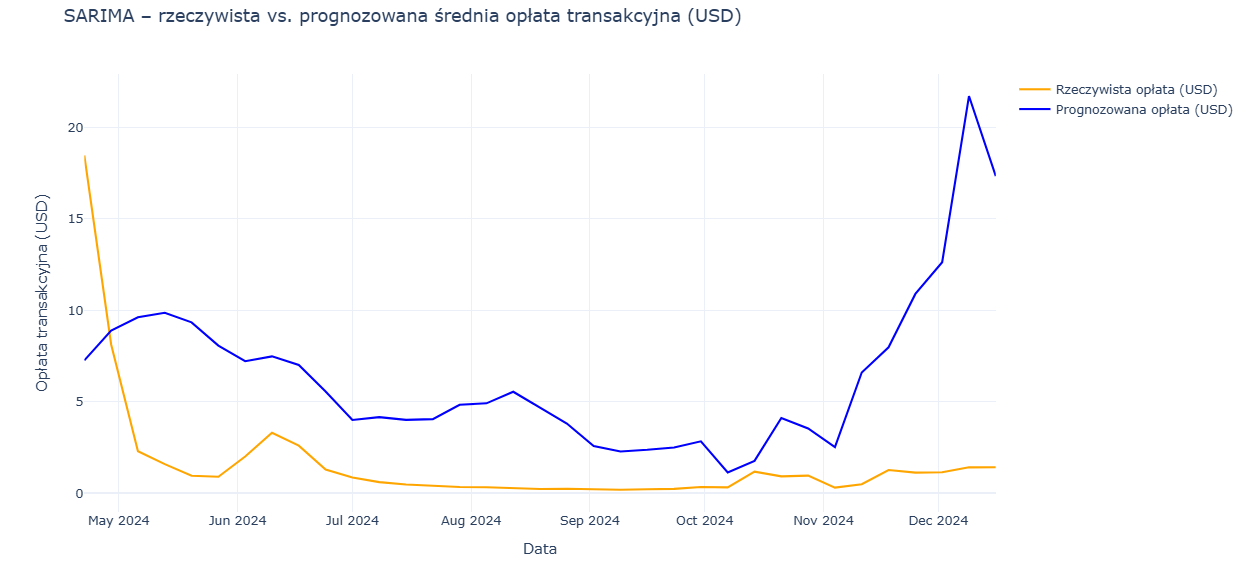
\includegraphics[width=0.95\textwidth]{../VSC_screeny/SARIMA_USD.PNG}
	\caption{SARIMA – rzeczywista vs. prognozowana opłata transakcyjna (USD)}
	\label{fig:SARIMAUSD}
	\end{figure}
	
	\begin{lstlisting}[language=Python,mathescape=true,caption=Wyniki predykcji SARIMA na zbiorze testowym,label=wynikiSARIMA]
	Test RMSE: 0.95752
	Test $R^2$: -0.7579
	\end{lstlisting}

Wartość RMSE wynosząca około 0.95752 wskazuje na wysoką przeciętną różnicę między prognozą a rzeczywistą wartością opłat wyrażoną w BTC, co sugeruje znaczną niedokładność modelu SARIMA dla badanego okresu. Ponadto, wartość współczynnika determinacji $R^2$ równa -0.7579 oznacza, że model nie jest w stanie poprawnie wyjaśnić zmienności obserwowanej w danych testowych, generując prognozy o niższej jakości niż prosta średnia.

\begin{figure}[H]
    \centering
    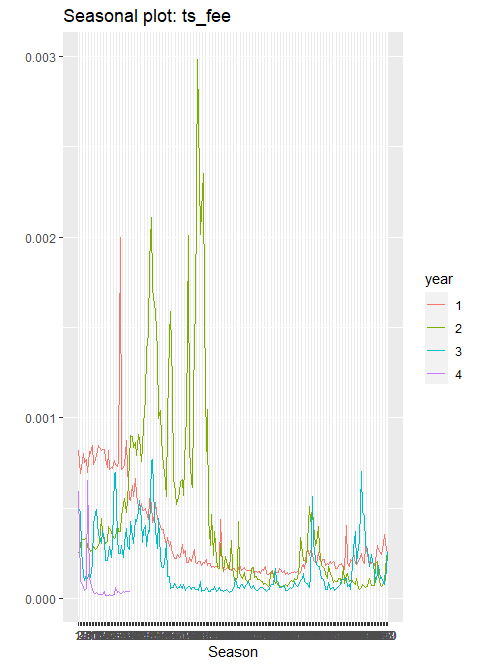
\includegraphics[width=0.55\textwidth]{../VSC_screeny/ggseasonplot_ts_fee.png}
    \caption{Sezonowy wykres średnich opłat transakcyjnych w kolejnych cyklach halvingu}
    \label{fig:ggseasonplot}
\end{figure}

W celu zrozumienia ograniczeń predykcyjnych modelu, przeanalizowano wykres sezonowości (\figurename~\ref{fig:ggseasonplot}). Zauważalny jest wyraźny wzorzec - podwyższone poziomy opłat w pierwszych oknach po halvingu, stopniowy spadek w środkowej części cyklu oraz tendencja do ponownego wzrostu w końcowej fazie. Jednak kształt tej zależności oraz poziom opłat różni się istotnie pomiędzy poszczególnymi cyklami, co sugeruje, że nie występuje ścisła powtarzalność sezonowa, a zmiany w strukturze opłat transakcyjnych mogą być wynikiem dodatkowych czynników zewnętrznych, takich jak zmiany aktywności sieci, wydarzenia rynkowe lub postęp technologiczny.

Dodatkowe spojrzenie daje wykres autokorelacji opóźnień (lag plot, \figurename~\ref{fig:lag_ts_fee}), przygotowany po zróżnicowaniu szeregu czasowego. Na wykresie tym, pomimo uwzględnienia 21 opóźnień odpowiadających okresowi halvingu (210 tysięcy bloków, czyli sezonowość użyta w modelu SARIMA), nie widać wyraźnego wzorca czy powtarzalnych struktur. Wskazuje to, że w analizowanym szeregu czasowym brak jest typowej, silnej sezonowości o dokładnie takim okresie, jest to raczej bardziej złożony i nieregularny proces, w którym powtarzalność nie jest pełna ani przewidywalna.

\begin{figure}[H]
    \centering
    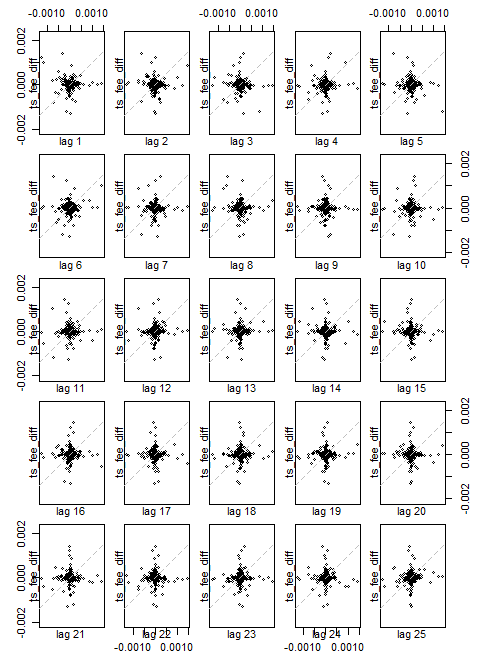
\includegraphics[width=0.55\textwidth]{../VSC_screeny/lagplot_fee_diff.png}
    \caption{Lag plot po zróżnicowaniu szeregu czasowego opłat transakcyjnych}
    \label{fig:lag_ts_fee}
\end{figure}

Wnioski płynące z tych analiz wskazują, że struktura sezonowa powiązana z halvingami jest niestabilna i~poddana wpływom czynników zewnętrznych, a cykle nie powtarzają się w identyczny sposób. Dodatkowo, w szeregu występują silne, nieprzewidywalne skoki opłat, co dodatkowo utrudnia dokładne modelowanie szeregów czasowych prostymi narzędziami, takimi jak SARIMA. Brak wyraźnych sygnałów sezonowości w~lagach potwierdza, że mechanizm kształtowania się opłat transakcyjnych jest złożony i wykracza poza sam cykl halvingowy.

Analiza ta potwierdza, że nawet uwzględnienie sezonowości i cyklicznych zmian wynikających z halvingów nie gwarantuje wystarczająco precyzyjnych wyników dla prognozowania opłat transakcyjnych. Wskazuje to na potrzebę uwzględnienia dodatkowych zmiennych lub zastosowania bardziej zaawansowanych metod modelowania.

	\subsection{Porównanie regresji liniowej i modelu SARIMA}
	\hspace*{\parindent}Pomimo zastosowania dwóch różnych metod modelowania jednowymiarowego: regresji liniowej oraz modelu SARIMA, uzyskane wyniki jednoznacznie wskazują na istotne ograniczenia predykcyjne związane z prognozowaniem opłat transakcyjnych wyłącznie na podstawie numeru bloku. Wartość współczynnika determinacji ($R^2$) dla regresji liniowej wyniosła jedynie 0.0212, co potwierdza bardzo słabą zdolność tego modelu do wyjaśniania zmienności danych. Jeszcze słabszy rezultat uzyskano w przypadku modelu SARIMA, dla którego $R^2$ przyjął ujemną wartość ($-0.7579$). Taki wynik oznacza, że model szeregów czasowych okazał się mniej skuteczny niż prosta regresja liniowa, która uwzględniała jedynie liniowy trend zmian opłat w funkcji numeru bloku.
	
	Bardzo niska skuteczność prognozowania może wynikać ze specyfiki wybranego predyktora. Numer bloku, mimo że pozwala modelować pewne trendy długoterminowe, nie zawiera wystarczającej ilości informacji o dynamice sieci, zmianach technologicznych czy czynnikach ekonomicznych (jak wahania kursu Bitcoina, wzrost aktywności użytkowników czy zmiany w polityce opłat). W szczególności model SARIMA, wymagający precyzyjnego określenia wzorca sezonowości, może nie być adekwatny do opisu tak złożonego i niestabilnego zjawiska, jakim są opłaty w sieci Bitcoin.

Jednak podejście jednowymiarowe może mieć zastosowanie w określonych przypadkach praktycznych. Przede wszystkim sprawdzi się ono tam, gdzie dostęp do pełnych danych o transakcjach jest ograniczony lub niemożliwy - na przykład w szybkich aplikacjach podglądowych, dashboardach czy prostych automatycznych szacunkach opłat na etapie wstępnym. Może także służyć do wstępnej oceny kierunku długoterminowego trendu, zwłaszcza gdy nie jest wymagana wysoka dokładność predykcji.

Podsumowując, dla osiągnięcia wyższej precyzji prognoz opłat transakcyjnych w sieci Bitcoin zaleca się korzystanie z bardziej złożonych modeli wielowymiarowych, które uwzględniają szeroki zestaw cech wejściowych. Modele jednowymiarowe, bazujące wyłącznie na numerze bloku, powinny być traktowane jako narzędzie poglądowe, pomocne w sytuacjach braku dostępu do szczegółowych danych lub przy szybkiej, orientacyjnej analizie trendu opłat.

	\chapter*{Podsumowanie}
	\hspace*{\parindent} Celem pracy była analiza oraz prognozowanie opłat transakcyjnych w sieci Bitcoin, uwzględniając zarówno aspekty techniczne (np. struktura bloków, konfiguracja węzła Bitcoin Core) jak i ekonomiczne (np. wpływ ceny Bitcoina na koszt transakcji). Zaprezentowano także proces przygotowania i przetwarzania obszernego zbioru 			danych, obejmującego zarówno informacje on-chain (m.in. \textit{block\_height}, \textit{fee}, \textit{miner\_reward}), jak i~dane rynkowe (historyczne wartości cenowe). Omówiono automatyzację pobierania bloków z wykorzystaniem Bitcoin RPC, wstępne czyszczenie i~transformację danych, a~także strategię doboru istotnych cech.

	W części analitycznej i prognostycznej porównano różne modele regresyjne: od regresji liniowej i jej wariantów (\textit{Ridge}, \textit{ElasticNet}), przez algorytmy oparte na drzewach decyzyjnych (\textit{Random Forest}, \textit{XGBoost}), aż po model szeregów czasowych SARIMA. Testy modeli wielowymiarowych realizowano przy wykorzystaniu szerokiego zbioru zmiennych wejściowych, natomiast w modelach jednowymiarowych (regresja liniowa oraz SARIMA) wykorzystywano wyłącznie numer bloku jako predyktor. Takie podejście pozwoliło rzetelnie porównać skuteczność predykcji w zależności od dostępności i~zakresu danych wejściowych.
	
	Wyniki jednoznacznie wykazały, że modele wielowymiarowe, szczególnie algorytmy zespołowe, takie jak XGBoost najlepiej radzą sobie z przewidywaniem wysokości opłat transakcyjnych, przewyższając pod względem trafności zarówno modele liniowe, jak i~model SARIMA w wariancie jednowymiarowym. Ręczne dostrajanie hiperparametrów nie dawało istotnych korzyści, natomiast zastosowanie GridSearchCV pozwoliło na optymalizację parametrów i poprawę jakości predykcji.

	Podejście jednowymiarowe, choć znacznie prostsze i możliwe do zastosowania w sytuacjach ograniczonego dostępu do danych (np. szybka estymacja, brak szczegółowych cech transakcyjnych), okazało się istotnie mniej skuteczne. Modele te praktycznie nie wyjaśniały zmienności opłat, a wartości współczynnika determinacji $R^2$ (ok. 2\% dla regresji liniowej, wartość ujemna dla SARIMA) wskazują na ograniczoną przydatność tej klasy rozwiązań w zastosowaniach wymagających precyzyjnych prognoz.

	Uzyskane wyniki mają jednak praktyczne znaczenie zarówno dla użytkowników sieci Bitcoin, którzy dążą do optymalizacji kosztów transakcji, jak i dla podmiotów oferujących usługi kryptowalutowe. Obserwacje dotyczące wpływu halvingów, dynamiki opłat i zmian cen Bitcoina dostarczają dodatkowych wniosków, które mogą wzbogacić dyskusję na temat skalowalności i przyszłości tej kryptowaluty.

	Warto zaznaczyć, że nawet najlepszy z modeli wielowymiarowych osiągnął stosunkowo niską wartość $R^2$ na poziomie ok. 23\% na zbiorze testowym, co pokazuje, iż prognozowanie opłat transakcyjnych w sieci Bitcoin pozostaje wyzwaniem, niezależnie od stopnia złożoności modelu. Sieć jest bowiem silnie podatna na dynamiczne wahania rynku i czynniki zewnętrzne, takie jak reakcje medialne czy decyzje kluczowych uczestników ekosystemu. Dla lepszej trafności predykcji warto w przyszłości rozważyć zastosowanie głębokich sieci neuronowych, hybrydowych podejść łączących modele zespołowe z modelami sieciowymi, a także wzbogacenie zbioru danych o wskaźniki nastrojów rynkowych czy sygnały pochodzące z analizy sentymentu.

	Autor za własny wkład pracy uważa przede wszystkim opracowanie kompleksowego podejścia do pobierania i przetwarzania danych z sieci Bitcoin przy użyciu węzła Bitcoin Core oraz automatyzacji (Bitcoin RPC, skrypty w Pythonie), wdrożenie narzędzi do eksploracji, przetwarzania i analizy danych (w tym inżynierii cech i skalowania), a także przeprowadzenie licznych eksperymentów z różnymi modelami regresyjnymi zarówno jedno, jak i wielowymiarowymi wraz z dostrajaniem hiperparametrów. Wszystkie te elementy składają się na istotny wkład w rozwój narzędzi analitycznych służących badaniu dynamiki kosztów transakcyjnych w sieci Bitcoin.
	\addcontentsline{toc}{chapter}{Podsumowanie}

	\begin{thebibliography}{3}
		\addcontentsline{toc}{chapter}{Bibliografia}
		\bibitem{kaspersky} https://www.kaspersky.com/resource-center/definitions/what-is-cryptocurrency. Dostęp: 21.03.2025.
		\bibitem{kanga} https://kanga.exchange/ Dostęp: 01.07.2025.
		\bibitem{bitcoin} A. Antonopoulos, D. Harding. Bitcoin. Wszystko, co musisz wiedzieć o programowaniu z użyciem otwartego łańcucha bloków. Wydanie III, 2024.
		\bibitem{Piotrowska} A. Piotrowska. 	Bitcoin. Płatnicze i inwestycyjne zastosowania kryptowaluty. Wydanie I, 2018.
		\bibitem{Nakamoto2008} Satoshi Nakamoto. Bitcoin: A Peer-to-Peer Electronic Cash System. 2008.
		\bibitem {fees} https://www.bitcoin.com/get-started/what-are-crypto-network-fees/. \\Dostęp: 21.03.2025.
		\bibitem{tangem} Tangem Team. Bitcoin Transaction Fees. Tangem Blog, 2021. 
		\bibitem{mempool} FAQ Mempool Documentation, 2023. https://mempool.space/docs/faq
		\bibitem{learnmeabitcoin} Greg Walker. Learn Me A Bitcoin, 2021. https://learnmeabitcoin.com/technical/tr- ansaction/fee/ Dostęp: 21.03.2025.
		\bibitem{hardfork} https://cryptomus.com/pl/blog/what-is-a-hard-fork-in-cryptocurrency \\Dostęp: 01.07.2025.
		\bibitem{MontgomeryPeckVining2012} Montgomery, D. C., Peck, E. A., \& Vining, G. G. Introduction to Linear Regression Analysis. 5th edition. (2012).
		\bibitem{Cucuringu2019} Cucuringu, M. Lecture 8b: LASSO and Ridge regression. Foundations of Data Science. (2019). https://www.stats.ox.ac.uk/~cucuring/LASSO\_Ridge.pdf Dostęp: 21.03.2025.
		\bibitem{Baladram2024} Baladram, S. Decision Tree Regressor, Explained: A Visual Guide with Code Examples. (2024).
		\bibitem{ibm} https://www.ibm.com/think/topics/random-forest. Dostęp: 21.03.2025.
		\bibitem{xgboost} https://datascience.eu/pl/programowanie-komputerowe/xgboost/. \\Dostęp: 21.03.2025.
		\bibitem{bitcoinCoreArchitecture}https://www.blockchain.com/explorer/charts/market-price. Dostęp: 21.03.2025.
		\bibitem{bitcoinPrice}https://cypherpunks-core.github.io/bitcoinbook/ch03.html. Dostęp: 21.03.2025.
	\end{thebibliography}
	\thispagestyle{empty}
\setlength{\parindent}{0in}
\setlength{\parskip}{0em}

\textbf{POLITECHNIKA RZESZOWSKA} \hfill Rzeszów, 2025 \\
\textbf{im. Ignacego Łukasiewicza} \\
\textbf{WYDZIAŁ MATEMATYKI I FIZYKI STOSOWANEJ} \\

\begin{center}
	\textbf{STRESZCZENIE  PRACY  DYPLOMOWEJ }
\end{center}

\textbf{Tytuł:} Analiza i prognozowanie opłat transakcyjnych sieci Bitcoina \\
\textbf{Autor:} inż. Daniel Krzysik \\
\textbf{Promotor:} dr inż. Dawid Jaworski \\
\textbf{Słowa klucze:} Bitcoin, blockchain, opłaty transakcyjne\\

Celem niniejszej pracy była analiza i prognozowanie opłat transakcyjnych w sieci Bitcoin. Przeprowadzono wstępną eksplorację danych blockchaina, pozyskanych bezpośrednio z węzła Bitcoin Core, a następnie przygotowano dane do dalszego przetwarzania. Zastosowano podejście zarówno wielowymiarowe, jak i jednowymiarowe wykorzystując, klasyczne algorytmy regresyjne, modele drzew decyzyjnych oraz model szeregów czasowych SARIMA. Uzyskane wyniki mogą wspierać podejmowanie decyzji przez użytkowników Bitcoina oraz stanowić podstawę do dalszych badań nad modelowaniem zjawisk blockchain.


% Wstawienie pionowej przestrzeni do połowy strony
\vfill
$$\noindent\rule{\textwidth}{2pt}$$
\vfill

\textbf{RZESZOW UNIVERSITY OF TECHNOLOGY} \hfill Rzeszów, 2025 \\
\textbf{FACULTY OF MATHEMATICS AND APPLIED PHYSICS } \\

\begin{center}
	\textbf{DIPLOMA THESIS ABSTRACT}
\end{center}

\textbf{Title:} Analysis and Forecasting of Bitcoin Network Transaction Fees\\
\textbf{Author:} Eng. Daniel Krzysik \\
\textbf{Supervisor:}  Dr Eng. Dawid Jaworski \\
\textbf{Key words:} Bitcoin, blockchain, transaction fees\\

The aim of this thesis was to analyze and forecast transaction fees in the Bitcoin network. An initial exploration of blockchain data obtained directly from the Bitcoin Core node was conducted, followed by data preprocessing. Both multivariate and univariate approaches were applied, using classical regression algorithms, decision tree models, and the SARIMA time series model. The obtained results may support decision-making by Bitcoin users and constitute a basis for further research on modeling blockchain phenomena.
	
	
	\end{document}

	
